%!TeX spellcheck = en-GB
\documentclass{entcs}
\usepackage{entcsmacrosasb}
\usepackage{graphicx}
\usepackage{amsmath}
\usepackage{calc}
\usepackage{mathtools}
\usepackage{kappa}
\usepackage{xypic}
\usepackage{subfigure}
\usepackage{stmaryrd}
\usepackage{boolean}
\sloppy
% The following is enclosed to allow easy detection of differences in
% ascii coding.
% Upper-case    A B C D E F G H I J K L M N O P Q R S T U V W X Y Z
% Lower-case    a b c d e f g h i j k l m n o p q r s t u v w x y z
% Digits        0 1 2 3 4 5 6 7 8 9
% Exclamation   !           Double quote "          Hash (number) #
% Dollar        $           Percent      %          Ampersand     &
% Acute accent  '           Left paren   (          Right paren   )
% Asterisk      *           Plus         +          Comma         ,
% Minus         -           Point        .          Solidus       /
% Colon         :           Semicolon    ;          Less than     <
% Equals        =3D           Greater than >          Question mark ?
% At            @           Left bracket [          Backslash     \
% Right bracket ]           Circumflex   ^          Underscore    _
% Grave accent  `           Left brace   {          Vertical bar  |
% Right brace   }           Tilde        ~

% A couple of exemplary definitions:

\newcommand{\map}[2]{#2}
\newcommand{\todo}[1]{{\huge\textcolor{red}{#1}}}
\newcommand{\todoo}[1]{{\large\textcolor{green}{#1}}}
\newcommand{\keep}[3]{#1{#2}{#3}}
\letboolval{\explainweakembedding}{\FALSE}
\newcommand{\binomial}[2]{{{#2}\choose{#1}}}
\newcommand{\validannotations}[1][EP]{\llbracket EP \rrbracket}
\newcommand{\realisationsaux}[2][EP]{\llbracket #2 \rrbracket_{#1}}
\newcommand{\realisations}[1][\phi]{\realisationsaux{#1}}
\newcommand{\canonic}{\bigcup \realisations}
\newcommand{\card}[1]{\sharp#1}
\newcommand{\Nat}{{\mathbb N}}
\newcommand{\Real}{{\mathbb R}}
\newcommand{\eps}[1]{}
\newcommand{\freesymbol}{\dashv}
\newcommand{\freeindex}[1]{%
\def\arga{#1}%
\if\arga0
\,\freesymbol\!
\else
\freesymbolrev\,
\fi}
\newcommand{\boundsymbol}{-}
\renewcommand{\bound}[1]{\boundsymbol}
\newcommand{\boundsymbolrev}{\boundsymbol}
\newcommand{\species}[3]{#1{0}A_#3#2{1}}
\newcommand{\rhodot}[3]{[\species{#1}{#2}{#3}]_e}
\newcommand{\conc}[3]{[\species{#1}{#2}{#3}]}
\newcommand{\concshort}[1]{[#1]}
\newcommand{\eg}{e.g.~}
\newcommand{\ie}{i.e.~}
\newcommand{\graphsymb}{G}
\newcommand{\iso}{\approx}
\newcommand{\rembedding}[1][]{\xymatrix@C=0.35cm{{}\ar@{^{(}->}[r]^{#1}&{}}}
\newcommand{\lembedding}[1][]{\xymatrix@C=0.35cm{{}&\ar@{_{(}->}[l]_{#1}}}
\newcommand{\rlongembedding}[1][]{\xymatrix@C=0.7cm{{}\ar@{^{(}->}[r]^{#1}&{}}}
\newcommand{\llongembedding}[1][]{\xymatrix@C=0.7cm{{}&\ar@{_{(}->}[l]_{#1}}}
\newcommand{\rvlongembedding}[1][]{\xymatrix@C=1cm{{}\ar@{^{(}->}[r]^{#1}&{}}}
\newcommand{\lvlongembedding}[1][]{\xymatrix@C=1cm{{}&\ar@{_{(}->}[l]_{#1}}}
\newcommand{\rvvlongembedding}[1][]{\xymatrix@C=1.3cm{{}\ar@{^{(}->}[r]^{#1}&{}}}
\newcommand{\lvvlongembedding}[1][]{\xymatrix@C=1.3cm{{}&\ar@{_{(}->}[l]_{#1}}}
\newcommand{\lvvvlongembedding}[1][]{\xymatrix@C=1.8cm{{}&\ar@{_{(}->}[l]_{#1}}}
\newdir{|>}{!/4.5pt/\dir{|}*:(1,-.2)\dir^{>}*:(1,+.2)\dir_{>}}


\newcommand{\agentname}{\signaturesymb_{\textit{ag}}}
\newcommand{\sitename}{\signaturesymb_{\textit{site}}}
\newcommand{\linksite}{\signaturesymb_{\textit{ag-st}}}
\newcommand{\signaturesymb}{\Sigma}
\newcommand{\signaturetuple}{(\agentname,\sitename,\linksite)}
\newcommand{\bydef}{\stackrel{\scalebox{0.8}{\!\!$\scriptscriptstyle{\triangle}$}}{=}}
\newcommand{\agents}[1][\graphsymb]{\mathcal{A}_{#1}}
\newcommand{\type}[1][\graphsymb]{\textit{type}_{#1}}
\newcommand{\sites}[1][\graphsymb]{\mathcal{S}_{#1}}
\newcommand{\links}[1][\graphsymb]{\mathcal{L}_{#1}}
\newcommand{\ext}{\{\freesymbol{}\}}
\newcommand{\graphtuple}[1][]{(\agents[#1],\type[#1],\sites[#1],\links[#1])}
\newcommand{\graphtuplebis}[1][]{(\agents[#1]',\type[#1]',\sites[#1]',\links[#1]')}

\newcommand{\myfrac}[2]{\frac{\strut \displaystyle #1}{\strut \displaystyle #2}}
\newcommand{\diff}[1]{\myfrac{\mathrm{d}#1}{\mathrm{d}t}}
\newtheorem{myexample}[thm]{Example}
\newcommand{\cons}[3]{\textit{p\_cons}_{\mathcal{M}}(#1,#2,#3)}
\newcommand{\conset}[1]{\textit{Cons}_{\mathcal{M}}(#1)}
\newcommand{\prodterm}[3]{\textit{p\_prod}_{\mathcal{M}}(#1,#2,#3)}
\newcommand{\prodset}[1]{\textit{Prod}_{\mathcal{M}}(#1)}
\def\lastname{Boutillier, Faure de Pebeyre, Feret, }
\begin{document}
\begin{frontmatter}
  \title{Proving the absence of unbounded polymers in rule-based models} \author{Pierre Boutillier\thanksref{pbemail}}
  \address{Harvard Medical School, \\ Department of Systems Biology, Boston, MA 02115, USA}
  \author{Aur\'elie Faure de Pebeyre\thanksref{afemail}}
\address{Centre de recherche interdisciplinaire, 75004 Paris, France}
\address{INRIA, \\ Centre de recherche INRIA de Paris, 75 012 Paris, France}
\address{D\'{e}partement d'informatique de l'\'{E}cole normale sup\'{e}rieure,\\
\'Ecole normale sup\'erieure, CNRS, PSL Research University,
75 005 Paris, France}
  \author{J\'{e}r\^{o}me Feret\thanksref{jfemail}}
  \address{INRIA, \\ Centre de recherche INRIA de Paris, 75 012 Paris, France}
  \address{D\'{e}partement d'informatique de l'\'{E}cole normale sup\'{e}rieure,\\
  \'Ecole normale sup\'erieure, CNRS, PSL Research University,
  75 005 Paris, France}
\thanks[pbemail]{Email:
    \href{mailto:pierre\_boutillier@hms.harvard.com} {\texttt{\normalshape
        pierre\_boutillier@hms.harvard.com}}}
\thanks[afemail]{Email:
            \href{mailto:aurelie.faure@cri-paris.org} {\texttt{\normalshape
        aurelie.faure@cri-paris.org}}}

\thanks[jfemail]{Email:
    \href{mailto:jerome.feret@ens.fr} {\texttt{\normalshape
        jerome.feret@ens.fr}}}
\begin{abstract}
%!TeX spellcheck = en-GB
Rule-based languages, such as Kappa and BNGL, allow for the description of very combinatorial models of interactions between proteins. A huge (when not infinite) number of different kinds of bio-molecular compounds may arise
 due to proteins with multiple binding and phosphorylation sites. Knowing beforehand whether a model may involve an infinite number of different kinds of bio-molecular compounds is crucial for the modeller. On the first hand, having an infinite number of kinds of bio-molecular compounds is sometimes a hint for modelling flaws: forgetting to specify
the conflicts among binding rules is a common mistake. On the second hand,
it impacts the choice of  the semantics for the models (among stochastic, differential, hybrid).

In this paper, we introduce a data-structure to abstract the potential unbounded polymers that may be formed in a rule-based model. This data-structure is a graph, the nodes and the edges of which are labelled with patterns. By construction,  every potentially unbounded polymer is associated to at least one cycle in that graph. This data-structure has two main advantages. Firstly, as opposed to site-graphs, one can reason about cycles without enumerating them (by the means of Tarjan's algorithm for detecting strongly connected components). Secondly, this data-structures may be combined easily with information coming from additional reachability analysis: the edges that are labelled with an overlap that is proved unreachable in the model may be safely discarded.

\end{abstract}
\begin{keyword}
  Rule-based modelling,
Polymers,
Static analysis,
Strongly connected components
\end{keyword}
\end{frontmatter}



\section{Introduction}

Rule-based languages, such as Kappa \cite{DBLP:journals/tcs/DanosL04} and BNGL
\cite{BNGL}, propose a transparent way to encode models of interactions between proteins.  Systems involving races for shared resources, different time- and concentration-scales, non linear feedback loops may be described by the means of rewrite rules. This allows for the description of very combinatorial models.   A huge (when not infinite) number of different kinds of bio-molecular compounds may arise due to the presence of scaffold and/or proteins with multiple binding and phosphorylation sites. The long term goal is then to understand how the collective behaviour of these proteins emerges from the mechanistic interactions between proteins.

Detecting whether such a model involve an infinite number of different kinds of bio-molecular compounds, is important. Often, the models come from a higher level of description \cite{DBLP:conf/cmsb/HarmerCLO17} or from automatic mining of the literature \cite{Gyori119834}. The presence of an infinite number of bio-molecular compounds is often a hint for a lack of specification. Namely, conflicts between potential bindings have not be specified enough and there is a need to refine the model. Sometimes the assembling of giant molecules is involved. In that later case, it is important to confirm that the model implements properly what the modeller has in mind.
The presence of an infinite number of distinct kinds of bio-molecular compounds also matters when choosing the most appropriate semantics for the models  (among stochastic, differential, hybrid).

In this paper, we introduce some graph structures to abstract the potential presence of unbounded polymers in a rule-based model. These graphs either cope for the potential succession of sites along chains of proteins in reachable bio-molecular compounds, or for the succession of bonds in these chains. They provide a sound and complete (with respect to the information provided by the contact map of the model) description of the potential binding between the sites of proteins.
The contact map encodes only non relational information: it cannot establish relationships about the different binding states of pairs of sites. Then, we show how to refine the graph of the potential successive links in bio-molecular compounds in order to refine it with the result of external relational static analyses \cite{DanosEtAl-VMCAI08,SASB2016,KaSa}. Such static analyses provide a list of patterns that are known unreachable. As a result, we get a sound, but not complete approach (the detection of unreachable patterns in a rule-base language is undecidable anyway \cite{kreyBig}) that may detect and prove that the set of non-isomorphic bio-molecular compounds of a model is finite, without executing the model.

The rest of the paper is organised as follows.
Sec.~\ref{sec:case-study} introduces some case study to provide intuitions about the property we want to infer, and to highlight pitfalls we will have to avoid. Sec.~\ref{sec:kappa} gives some reminders about Kappa.
In Sec.~\ref{sec:graphs}, we introduce two families of graph to decide whether or not the set of bio-molecular compounds that are compatible with a contact map is finite. We refine our approach to deal with black-listed patterns in Sec.~\ref{sec:refinement}.



\begin{figure}
  \subfigure[Contact map.]{%
  \begin{minipage}{0.25\linewidth}
      \label{fig:abc:cm}
  \centering\scalebox{0.6}{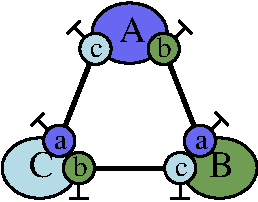
\includegraphics{generated_pictures/abc_contact_map.pdf}}\vspace*{2.5mm}\smallskip\\%
\end{minipage}
  }
  \subfigure[Triangle \agentfont{ABC}.]{%
  \begin{minipage}{0.25\linewidth}
    \label{fig:abc:triangle}
  \centering\scalebox{0.6}{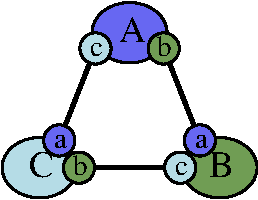
\includegraphics{generated_pictures/abc_triangle.pdf}}\vspace*{2.5mm}\smallskip\\%
\end{minipage}
  }
  \subfigure[A repeatable pattern.]{%
  \begin{minipage}{0.45\linewidth}
    \label{fig:abc:pattern}
    \vspace*{0.6cm}
  \centering\scalebox{0.6}{
\includegraphics{generated_pictures/abc_pattern.pdf}}\vspace*{0.5cm}\smallskip\\%
\end{minipage}}
\caption{The \agentfont{ABC} example.
The contact map  (Fig.\ref{fig:abc:cm}) specifies a typing discipline.
It displays every kind of protein and specifies their interfaces.
The contact map also provides the potential states for each site:
either free $\freesymbol$, or bound to another site (which is encoded as a link between pair of sites in the contact map).
In Fig.~\ref{fig:abc:triangle} is described a bio-molecular compound that is compatible with the contact map. Every instance of proteins belongs to the contact map. Their interfaces are the same as in the contact map.
Also any bond between two sites complies with one link explicitly written in the contact map.
Fig.~\ref{fig:abc:pattern} describes a repeatable pattern.
This pattern is compatible with the contact map and can be repeated in order to form arbitrarily large bio-molecular compounds.
}\label{fig:abc}
\end{figure}
\section{Case studies}
\label{sec:case-study}

In this section, we introduce some examples to explain intuitively why there may be an unbounded number of bio-molecular compounds in a rule-based model.  We also explain why naive approaches may fail in proving that the number of bio-molecular compounds is finite in a given model when it is the case,  while identifying the pitfalls that shall be avoided to achieve this goal.

\subsection{Elementary cycles}

\label{sec:triangle}

Let us start with a simple example. We consider a model involving three kinds of protein $A$, $B$, $C$. Each protein has two binding sites: the protein $A$ has the binding sites $b$ and $c$, the protein $B$ has the binding sites $a$ and $c$, and the protein $C$ has the binding sites $a$ and $b$. Each binding site may be free, or bound to another site. Only three kinds of bond are possible: the site $b$ of an instance of the protein $A$ may be bound to the site $a$ of an instance of the protein $B$; the site $c$ of an instance of the  protein $B$ may be bound to the site $b$ of an instance of the protein $C$; and the site $a$ of an instance of the protein $C$ may be bound to the site $c$ of a protein $A$.

These assumptions are summarised in a graph in Fig.~\ref{fig:abc:cm}. This graph is called the contact map of the model. It describes every kind of protein and every site in their interfaces. The potential state of each site is also indicated. In our model, every site may be free: they are all tagged with the symbol $\freesymbol$. Potential bonds are indicated by the means of non oriented edges between pairs of sites.  The contact map provides a typing discipline.
Every bio-molecular compound in our models shall satisfy the constraints the contact map is encoding about the interface of agents, the potential states of sites, and their potential bindings. An example of bio-molecular compound that is compatible with the contact map is drawn in Fig.~\ref{fig:abc:triangle}. This bio-molecular compound is made of three proteins \agent{A}{}, \agent{B}{}, and \agent{C}{}{} that are bound pair-wise so as to form a triangular shape.
In a bio-molecular compound, every site shall be exclusively either free, or bound to at most one other site. In general, a bio-molecular compound does not have to contain an instance of each kind of protein. Also it may contain several instances of some of them.

The contact map that is given in Fig.~\ref{fig:abc:cm} is compatible with an infinite number of different (i.e.~\emph{non isomorphic}) molecular compounds.
Indeed we show in Fig.~\ref{fig:abc:pattern}, a pattern
that may be repeated an unbounded number of times in order to form arbitrary many different bio-molecular compounds. This is tempting to relate the potential presence of an arbitrary number of different bio-molecular compounds to the one of a cycle in the contact map. However we shall see in the next examples that this intuition is misleading.


\begin{figure}
  \subfigure[Contact map.]{%
  \begin{minipage}{0.3\linewidth}
      \label{fig:self:cm}
  \centering\scalebox{0.6}{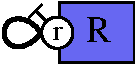
\includegraphics{generated_pictures/self_contact_map.pdf}}\vspace*{2.5mm}\smallskip\\%
\end{minipage}
  }
  \subfigure[Exhaustive list of bio-molecular compounds.]{%
  \begin{minipage}{0.6\linewidth}
    \label{fig:self:species}
  \centering\hfill\scalebox{0.6}{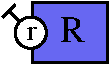
\includegraphics{generated_pictures/self_monomer.pdf}}\hfill\scalebox{0.6}{
\includegraphics{generated_pictures/self_dimer.pdf}}\hfill\mbox{}\vspace*{2.5mm}\smallskip\\%
\end{minipage}}
\caption{The example of a protein that may form monomers and dimers.
The contact map (e.g.~see Fig.~\ref{fig:self:cm}) contains a cycle, since the unique site of an instance of a  protein may be linked to the unique site of another instance of another protein. However, only once instance of this cycle may occur in a given bio-molecular compound and the number of bio-molecular compound remains bounded despite this cycle (e.g.~see Fig.~\ref{fig:self:species}).}
\end{figure}

\begin{figure}
  \subfigure[Contact map.]{%
  \begin{minipage}{0.45\linewidth}
      \label{fig:twoself:cm}
  \centering\scalebox{0.6}{
\includegraphics{generated_pictures/twoself_contact_map.pdf}}\vspace*{2.5mm}\smallskip\\%
\end{minipage}
  }
  \subfigure[A repeatable pattern.]{%
  \begin{minipage}{0.45\linewidth}
    \label{fig:twoself:pattern}
  \centering\scalebox{0.6}{
\includegraphics{generated_pictures/twoself_pattern.pdf}}\vspace*{2.5mm}\smallskip\\%
\end{minipage}}
\caption{An example of a protein with two sites \sitefont{a} and \sitefont{b} such that the site {\sitefont{a}}\;\; of a protein may be bound to the site \sitefont{a} of another protein and the site \sitefont{b} may be bound to the site \sitefont{b}\;\; of another protein.
The contact map (Fig.\ref{fig:twoself:cm}) contains two self-loops.
The pattern that is made of three proteins, the first two bound via their respective sites \sitefont{a} and the last two bound via their respective sites \sitefont{b} is a repeatable patterns. Thus, an infinite number of bio-molecular compounds is compatible with the contact map.  }
\end{figure}

\subsection{Self loops}
\label{sec:self-loop}
In this example we consider a model with only one kind of protein. This protein has a single site which may be either free, or bound to the unique site of another protein of the same kind. Roughly speaking proteins may form monomers  and dimers. These assumptions are encoded in the contact map that is given in Fig.~\ref{fig:self:cm}. We notice a cycle in this contact map (from the unique site of the protein to itself). Yet only the two bio-molecular compounds that are depicted in Fig.~\ref{fig:self:species} are compatible with this contact map:  there is a finite number of kinds of bio-molecular compound them despite the presence of a cycle in the contact map.

One could think that self-loops should not be considered as cycles when trying to prove the finiteness of the set of bio-molecular compounds of a model. Indeed whenever a molecular compound contains a bond that corresponds to a self-loop in the contact map, then both sites are necessarily  bound together and they are no longer available to form links with other sites. Yet the contact map that is given in Fig.~\ref{fig:twoself:cm} shows that it is unsafe in general  to discard self-loops from the contact map. In this example, we consider only one kind of protein with two sites. Each site may be either free, or bound to the same site of another instance of the protein. It is then possible to form a chain of three proteins (see Fig.~\ref{fig:twoself:pattern}) that may be repeated an arbitrary number of times in a bio-molecular compound.

\subsection{Conflicting bindings}
\label{sec:conflict}
\begin{figure}
  \subfigure[Contact map.]{%
  \begin{minipage}{0.25\linewidth}
      \label{fig:conflict:cm}
  \centering\scalebox{0.6}{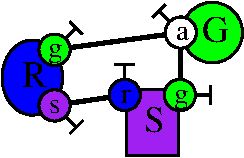
\includegraphics{generated_pictures/conflict_contact_map.pdf}}\vspace*{2.5mm}\smallskip\\%
\end{minipage}
  }
  \subfigure[Exhaustive list of bio-molecular compounds.]{%
  \begin{minipage}{0.74\linewidth}
    \label{fig:conflict:pattern}
  \scalebox{0.6}{\hspace*{2mm}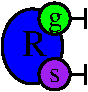
\includegraphics{generated_pictures/conflict_r.pdf}}%
  \hspace*{7mm}\scalebox{0.6}{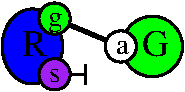
\includegraphics{generated_pictures/conflict_rg.pdf}}%
  \hspace*{7mm}\scalebox{0.6}{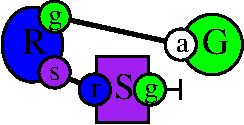
\includegraphics{generated_pictures/conflict_grs.pdf}}%
  \hspace*{7mm}\scalebox{0.6}{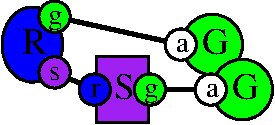
\includegraphics{generated_pictures/conflict_ggrs.pdf}}%

  \scalebox{0.6}{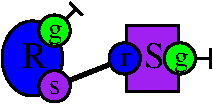
\includegraphics{generated_pictures/conflict_rs.pdf}}%
  \hspace*{3mm}\scalebox{0.6}{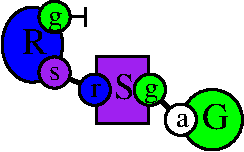
\includegraphics{generated_pictures/conflict_gbisrs.pdf}}%
  \hspace*{3mm}\scalebox{0.6}{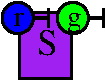
\includegraphics{generated_pictures/conflict_s.pdf}}%
  \hspace*{3mm}\scalebox{0.6}{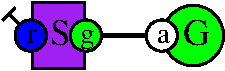
\includegraphics{generated_pictures/conflict_gs.pdf}}%
  \hspace*{3mm}\scalebox{0.6}{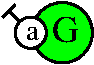
\includegraphics{generated_pictures/conflict_g.pdf}}%

\end{minipage}}
\caption{An example of a protein with a site that may be bound to two different kinds of site. As drawn in the contact map (e.g.~see Fig.~\ref{fig:conflict:cm}), the site of the protein \agentfont{G} may be either free, bound to the site \sitefont{g} of the protein \agentfont{R}, or bound to the site \sitefont{g} of the protein \agentfont{S}. The cycle in the contact map does not induce an infinite number of different bio-molecular compounds (e.g.~see Fig.~\ref{fig:conflict:pattern}). }
\end{figure}

In this example, we consider three kinds of protein \agentfont{G}, \agentfont{R}, and \agentfont{S}. The proteins of kind \agentfont{G} have a single site; the proteins of kind \agentfont{R} have two sites \sitefont{g} and \sitefont{s}; and the proteins of kind \agentfont{S} have two sites \sitefont {g} and \sitefont{r}. Proteins \agentfont{R} and \agentfont{S} may bind to each-other via their respective sites \sitefont{s} and \sitefont{r}.
The unique site of proteins \agentfont{G} may bind either to the site \sitefont{g} of an instance of the protein \agentfont{R}, or to the site \sitefont{g} of an instance of the protein \agentfont{S}. Thus, there is a competition, or a conflict, on the site of the protein \agentfont{G}.

The contact map for this example is provided in Fig.~\ref{fig:conflict:cm}.
We notice that the competition on the site of the protein \agentfont{G} belongs to a cycle in this contact map. Yet, in a given bio-molecular compound,
the site of each instance of \agentfont{G} is either free, or bound to at most one site. Thus the cycle of the contact map is not realisable
in a concrete bio-molecular compound. In Fig.~\ref{fig:conflict:pattern}, we enumerate all the bio-molecular compounds that are compatible with the constraints encoded in the contact map. There is a finite amount of them, despite the presence of a cycle in the contact map.


\subsection{Early events in the epidermic growth factor pathway}

\label{sec:egfr}

\begin{figure}[t]
  \begin{minipage}{0.4\linewidth}%
\subfigure[Contact map.]{%
\label{fig:egfr:cm}
\begin{minipage}{\linewidth}%
\begin{center}
  \scalebox{0.4}{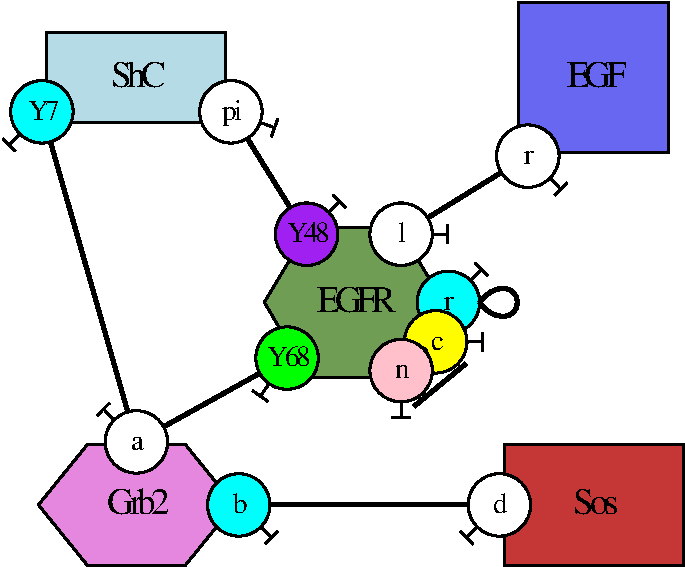
\includegraphics{generated_pictures/contact_map.pdf}}\vspace*{2.5mm}\smallskip\\%
\end{center}
\end{minipage}%
}
\subfigure[A repeatable pattern.]{%
\label{fig:egfr:pattern}
\begin{minipage}{\linewidth}%
\begin{center}
  \scalebox{0.4}{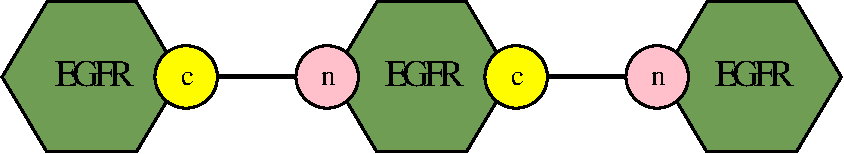
\includegraphics{generated_pictures/egfr_egfr_egfr.pdf}}\vspace*{2.5mm}\smallskip\\%
\end{center}
\end{minipage}%
}\end{minipage}
\subfigure[A bio-molecular compound.]{%
\label{fig:egfr:species}
\begin{minipage}{0.59\linewidth}%
\begin{center}\scalebox{0.4}{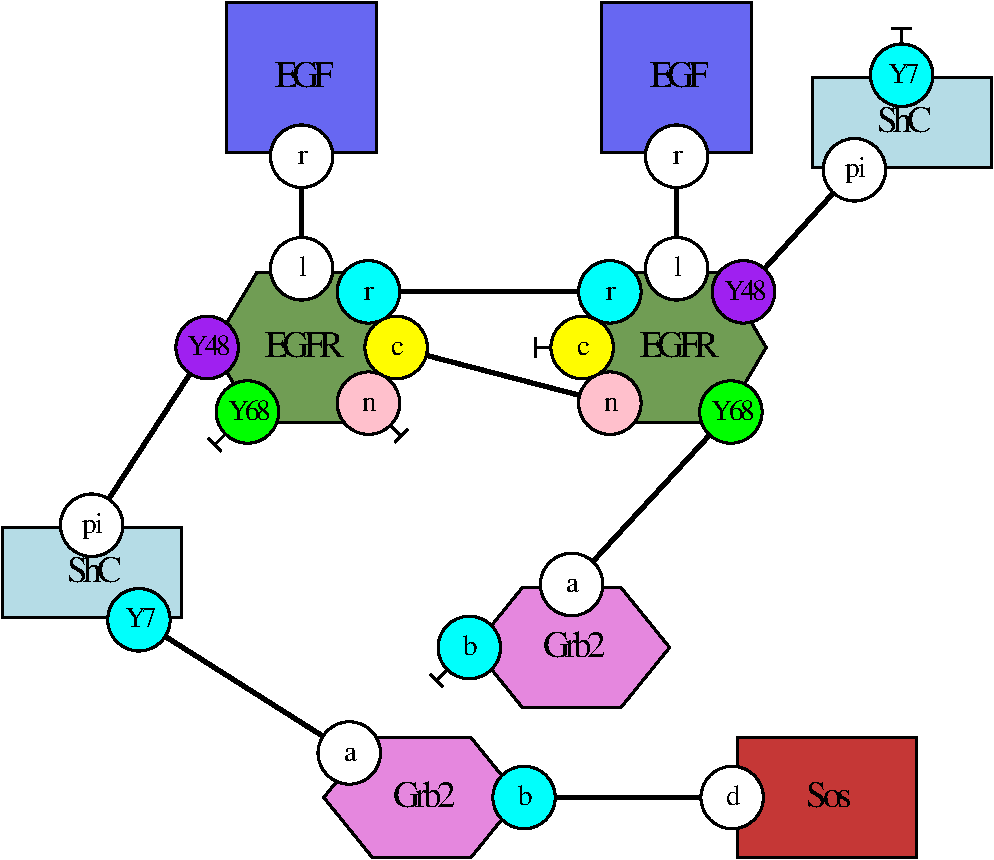
\includegraphics{generated_pictures/species.pdf}}\smallskip\\\end{center}%
\end{minipage}}
\caption{The example of the early events in the epidermic growth factor \cite{Blinov-2006-ANM}. In Fig.~\ref{fig:egfr:cm} is drawn the contact map. Compared to the original model in BNGL, we have omitted phosphorylation states, since they have no impact on the binding topology. We have also
added two sites in the receptor to model the asymetric bond between receptors \agentfont{EGFR} in dimers.
The model is constrained by the following property: whenever the site \sitefont{c} of a receptor \agentfont{EGFR} is bound, then its site \sitefont{r} is bound as well, and both sites are bound to the same instance
of protein. The contact map is compatible with the repeatable pattern that is given in Fig.~\ref{fig:egfr:pattern}. Yet this pattern does not satisfy the additional constraint. Indeed the model has only a finite set of different bio-molecular compounds. In Fig.~\ref{fig:egfr:species} is given an example of a typical bio-molecular compound.}
\label{fig:egfr}
 \end{figure}

So far, we have considered only toy examples, since we tried to understand which conditions on a contact map are necessary to induce only a finite number of bio-molecular compounds. In Fig.~\ref{fig:egfr}, we consider
a model for the early events in the integration of the epidermic growth factor (EGF) \cite{Blinov-2006-ANM}. In this model, the acquisition of the protein \agentfont{Sos} by the membrane of the cell is made in several steps.
Firstly a pair of receptors \agentfont{EGFR} on the membrane of the cell shall be activated by the ligands \agentfont{EGF}. Once bound to their respective ligands, they can form a dimer thanks to a symmetric bond via their respective sites
\sitefont{r}. Compared to the BNGL model of \cite{Blinov-2006-ANM}, asymmetric bonds between receptors are also considered. To stabilise dimers, pairs of receptors that are bound via their sites \sitefont{r} form an asymmetric binding by connecting the site \sitefont{c} of one receptor to the site \sitefont{n} of the other receptor. The symmetric bond in a dimer cannot be released in the presence of an asymmetric one. As a consequence, whenever the site \sitefont{c} of a receptor is bound to the site \sitefont{n} of another receptor, these receptors are also connected by a symmetric bond. This property can be inferred
by the static analysis that is described in \cite{SASB2016,KaSa}.
Each receptor in a dimer may activate the sites \sitefont{Y48} and \sitefont{Y68} of the other receptor (since we focus only on the binding topology, we omit the details about these activations which are performed by the means of phosphorylation). The site \sitefont{Y68} may bind to the protein \agentfont{Grb2}, which may be, or not, bound to the protein
\agentfont{Sos}. The site \sitefont{Y48} connects to the protein \agentfont{Grb2} indirectly, thanks to the adapter protein \agentfont{Shc}.

It is worth noticing that the contact map, that is depicted in Fig.~\ref{fig:egfr:cm} does not provide all the information about the model.
The constraints on the sites \sitefont{c}, \sitefont{n}, and \sitefont{r} emerge from some mechanisms that are described by the means of rules.
Rules are omitted here so as to focus on the topology of the potential bindings between the sites of proteins. Yet some additional constraints may be provided as a list of forbidden patterns. This way, we assume that the bio-molecular compounds of our model are the ones that are compatible with the contact map and that does not contain black-listed patterns.

Interestingly, the contact map of the EGF model (e.g.~see \ref{fig:egfr:cm})
contains both issues that we have pointed out in Sec.~\ref{sec:self-loop} and in Sect.~\ref{sec:conflict}. Indeed, the site \site{r}{}{} of a receptor may be bound to the site \site{r}{}{} of another receptor. Moreover there is a conflict on the site \site{a}{}{} of the protein \agent{Grb2}{} which may be bound to the receptor directly
or via an adapter protein. Another issue is raised by this model.
The constraints provided by the contact map are not enough to ensure the finiteness of the set of the different bio-molecular compounds. Indeed,
the pattern that is provided in Fig.~\ref{fig:egfr:pattern} is compatible with the contact map, and could be repeated an unbounded number of times to form an infinite number of different bio-molecular compounds. Nevertheless, this pattern is not compatible with the additional constraints about symmetric and assymetric bindings in dimers: there is only a finite number of different bio-mollecular compounds that satisfies both
the constraints from the contact map and the additional constraint.
In Fig.~\ref{fig:egfr:species}, we provide a typical example of bio-molecular compound in the EGF model. This example is made of a dimer, with one site \sitefont{Y68} free, one site \sitefont{Y68} connected to a \agentfont{Grb2} not connected to a \agentfont{Sos}, one site \sitefont{Y48} connected to an adapter not connected to a \agentfont{Grb2}, and a site \sitefont{Y48} connected to a \agentfont{Sos}. In total, a dimer may be connected to up to four instances of \agentfont{Sos}.

On such a rather small model, it is possible to enumerate the different bio-molecular compounds thanks to reaction enumeration engines  \cite{BNGL,KaDe}. This model is made of $253$ kinds of bio-molecular compounds.
Taking into account phosphorylation states would lead to a model
with $932$ kinds of bio-molecular compounds. Nevertheless, enumeration engines do not scale to large combinatorial networks such as the longer version of the EGF model (including the interactions with the proteins Ras, Erk, and Mapk) that is described in \cite{DanosEtAl-CONCUR07} and that involves about $10^{19}$ different kinds of bio-molecular compounds \cite{DanosEtAl-VMCAI08} or as the model of the interactions found in the cytoplasmic portion of the Structural Interaction Network (cSIN) \cite{Deeds-et-al-plosone2012,Kim} that involves an infinite number of bio-molecular compounds.

We will design a well-suited data-structure to abstract the elementary repeatable patterns that are compatible with a contact map and with additional constraints.

\subsection{Clique}

In large combinatorial models, the set of elementary repeatable patterns
may not be represented explicitly. It is important to abstract it.

Let us consider the example of a clique of $n$ proteins.
We call a clique of $n$ proteins any $n$ kinds of protein such that each protein has exactly $n-1$ sites and that every pair of proteins of distinct kinds may be connected by exactly one pair of sites. The number of elementary repeatable patterns in a clique of $n$ proteins  is exponential with respect to $n$ (there is indeed $\frac{n!}{k!}$  elementary repeatable patterns with exactly $k+1$ proteins, for any $k$ such that $2\leq k \leq n$).
Thus they cannot be all enumerated. In this paper, we will instead compute exactly the set of bonds that may occur in repeatable patterns.
Our approach is based on the use of some graphs that are derived from the contact map, and for which edges correspond to the potential bonds in elementary repeatable patterns. We use Tarjan's algorithm \cite{tarjan} to compute the strongly connected components of these graphs. Our analysis is sound and complete with respect to the constraints that are encoded in the contact map: a bond may occur in a repeatable pattern that is compatible with a given  contact map if and only if it corresponds to an edge in a non trivial strongly connected component of the graph that is associated to this contact map. Moreover, it is possible to take into account additional constraints about the patterns that are proved to be unreachable by traditional static analysis \cite{SASB2016,KaSa}.

\emph{Outline.} The rest of the paper is organised as follows.
In Sec.~\ref{sec:kappa}, we give some reminders about Kappa.
We focus only on static reasoning about graphs. We do not introduce the notion of rules. We assume that
additional constraints about reachable patterns come from a black box that we do not describe in this paper. In Sec.~\ref{sec:graphs}, we introduce two notions of graphs: the graph of the sites and the graph of the potential links. Both notions can be used to reason about the finiteness of the set of bio-molecular compounds in a Kappa model. Yet we will see in Sec.~\ref{sec:refinement}, that the graph of the potential links may be refined to take into account the patterns that may be proved unreachable by an external tool.

















\section{Kappa}

\label{sec:kappa}

In this section, we give some reminders about Kappa.
We do not introduce the full semantics of Kappa. Instead, we introduce only the notions of site-graphs and of embeddings among them. We omit the notions of rules and of rule applications. We also omit internal states, since we focus on the topology of the potential bindings between proteins.   We refer to \cite{DBLP:journals/tcs/DanosL04,Feret_IJSI2013} for a more complete description of Kappa.

\subsection{Signature}

Firstly we define the signature of a model.
\begin{defn}[signature]
\label{def:signature}
A signature is a triple $\signaturesymb\bydef\signaturetuple$ where: \begin{enumerate}\item $\agentname$ is a finite set of agent types, \item $\sitename$ is a finite set of site identifiers; \item $\linksite\;:\;\agentname \rightarrow \wp(\sitename)$ is a site map.
\end{enumerate}\end{defn}


Agent types in $\agentname$ denote agents of interest, as kinds of protein for instance.
Site identifiers in $\sitename$ represent identified loci for capabilities of interactions.
Agent types $A\in\agentname$ are associated with sets of sites $\linksite(A)$ which may be linked.


\begin{myexample}[signature (model of the triangle)]
\label{ex:signature:abc}We define the signature for the model of the triangle
(e.g.~see Sec. \ref{sec:triangle}):
\begin{equation*}\signaturesymb\bydef\signaturetuple\end{equation*} where:
 \begin{enumerate}
 \item $\agentname \bydef \{\text{\agent{A}{}},\text{\agent{B}{}},\text{\agent{C}{}}\}$;
 \item $\sitename \bydef \{\text{\site{a}{}{}},\text{\site{b}{}{}},\text{\site{c}{}{}}\}$;
 \item $\linksite \bydef \map{%
 \begin{cases}
   \begin{array}{ccc}\agentname &\rightarrow & \wp(\sitename) \cr
   \text{\agent{A}{}}&\mapsto& \{\text{\site{b}{}{}},\text{\site{c}{}{}}\}\cr
   \text{\agent{B}{}}&\mapsto& \{\text{\site{a}{}{}},\text{\site{c}{}{}}\}\cr
   \text{\agent{C}{}}&\mapsto& \{\text{\site{a}{}{}},\text{\site{b}{}{}}\}\cr
\end{array}\end{cases}}{[\text{\agent{A}{}}\mapsto \{\text{\site{b}{}{}};\text{\site{c}{}{}}\},
\text{\agent{B}{}}\mapsto \{\text{\site{a}{}{}};\text{\site{c}{}{}}\},
\text{\agent{C}{}}\mapsto \{\text{\site{a}{}{}};\text{\site{b}{}{}}\}]}$.
 \end{enumerate}
%  The agent types \agent{A}{}, \agent{B}{}, and \agent{C}{} denote the three kinds of protein. Each instance of the protein \agent{A}{} has three sites the identifiers of which range from $1$ to $3$;
%  each instance of the protein \agent{B}{} has four sites the identifiers  of which range from $1$ to $4$; and each instance of the protein \agent{C}{} has two sites the identifiers of which range from $1$ to $2$.
\end{myexample}
\begin{myexample}[signature]
\label{ex:signature}We define the signature for the model of the early events in the epidermic growth factor (e.g.~see Sec.~\ref{sec:egfr})::
\begin{equation*}\signaturesymb\bydef\signaturetuple\end{equation*} where:
 \begin{enumerate}
 \item $\agentname \bydef \{\text{\agent{EGF}{}},\text{\agent{EGFR}{}},\text{\agent{Grb2}{}},\text{\agent{ShC}{}},\text{\agent{Sos}{}}\}$;
 \item $\sitename \bydef \{\text{\site{a}{}{}},\text{\site{b}{}{}},\text{\site{c}{}{}},
 \text{\site{d}{}{}},
\text{\site{n}{}{}},
 \text{\site{l}{}{}},
 \text{\site{pi}{}{}},
 \text{\site{r}{}{}},
 \text{\site{Y7}{}{}},\text{\site{Y48}{}{}},\text{\site{Y68}{}{}}\}$;
 \item $\linksite \bydef \map{%
 \begin{cases}
   \begin{array}{ccc}\agentname &\rightarrow & \wp(\sitename) \cr
   \text{\agent{EGF}{}}&\mapsto& \{\text{\site{r}{}{}}\}\cr
   \text{\agent{EGFR}{}}&\mapsto& \{\text{\site{c}{}{}},
  \text{\site{n}{}{}},
   \text{\site{l}{}{}},
   \text{\site{r}{}{}},
  \text{\site{Y48}{}{}},\text{\site{Y68}{}{}}\}\cr
\text{\agent{Grb2}{}}&\mapsto & \{\text{\site{a}{}{}},\text{\site{b}{}{}}\}\cr
\text{\agent{ShC}{}}&\mapsto &
\{\text{\site{pi}{}{},\site{Y7}{}{}}\}\cr
\text{\agent{Sos}{}}&\mapsto &
\{\text{\site{d}{}{}}\} \cr\end{array}\end{cases}}{\left[\begin{array}{l}\text{\agent{EGF}{}}\mapsto \{\text{\site{r}{}{}}\},
\text{\agent{EGFR}{}}\mapsto \{\text{\site{c}{}{}},
\text{\site{n}{}{}},
\text{\site{l}{}{}},
\text{\site{r}{}{}},
\text{\site{Y48}{}{}},\text{\site{Y68}{}{}}\},\cr
\text{\agent{Grb2}{}}\mapsto \{\text{\site{a}{}{}},\text{\site{b}{}{}}\},
\text{\agent{ShC}{}}\mapsto
\{\text{\site{pi}{}{},\site{Y7}{}{}}\},
\text{\agent{Sos}{}}\mapsto
\{\text{\site{d}{}{}}\}\end{array}\right]}$
 \end{enumerate}
%  The agent types \agent{A}{}, \agent{B}{}, and \agent{C}{} denote the three kinds of protein. Each instance of the protein \agent{A}{} has three sites the identifiers of which range from $1$ to $3$;
%  each instance of the protein \agent{B}{} has four sites the identifiers  of which range from $1$ to $4$; and each instance of the protein \agent{C}{} has two sites the identifiers of which range from $1$ to $2$.
\end{myexample}

\subsection{$\Sigma$-graphs and morphisms among $\Sigma$-graphs}


$\Sigma$-graphs are graphs. Their nodes are typed agents with some sites which may bear sets of binding states. Contact maps, patterns and bio-molecular compounds are specific kinds of $\Sigma$-graph.


\begin{figure}[t]
\subfigure[A morphism from $\graphsymb_{\Sigma}$ into $\graphsymb_{\textit{CM}}$.]{%
\label{fig:morphism}
\begin{minipage}{\linewidth}%
\vspace*{0.6cm}
\begin{center}\scalebox{0.4}{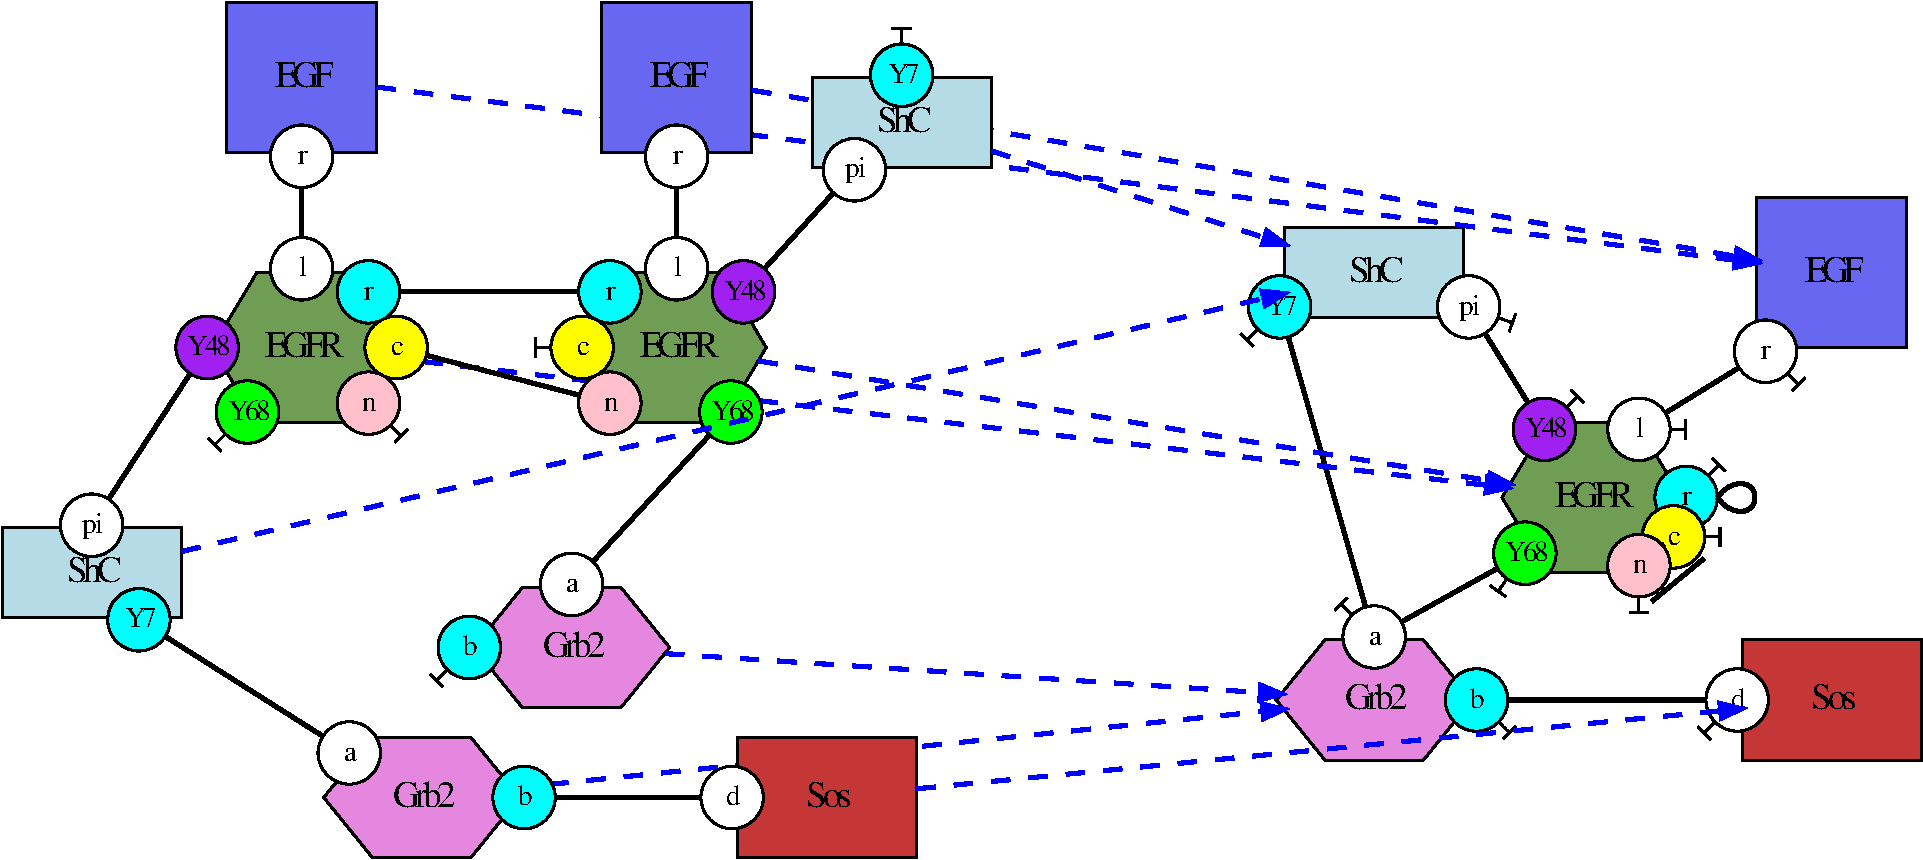
\includegraphics{generated_pictures/species_cm.pdf}}\smallskip\\%\vspace*{0.55cm}
\end{center}%
\end{minipage}}

\caption{Two $\Sigma$-graphs $\graphsymb_{\textit{CM}}$ and
$\graphsymb_{\textit{SP}}$, and a morphism from $\graphsymb_{\textit{CM}}$ to $\graphsymb_{\Sigma}$. The $\Sigma$-graph $\graphsymb_{\textit{CM}}$ is a contact map. It provides context-insensitive information about the potential state of each binding site. The $\Sigma$-graph $\graphsymb_{\textit{SP}}$ is a bio-molecular compounds. It containts several instances of some proteins.
Every site is documented in each protein instance and each site is either free, or bound to another site. The morphism between $\graphsymb_{\textit{CM}}$ and $\graphsymb_{\textit{SP}}$ smashes all
the proteins of the $\Sigma$-graph $\graphsymb_{\textit{SP}}$ according to their type. This is the unique morphism from the site graph $\graphsymb_{\textit{CM}}$ into the site-graph $\graphsymb_{\textit{SP}}$.
}
\label{fig:sigma-graphs}
\end{figure}

\begin{defn}[$\Sigma$-graphs]\label{def:summary}
A $\Sigma$-graph is a tuple $\graphsymb\bydef\graphtuple[G]$ where:
\begin{enumerate}
\item $\agents[G]\subseteq \mathbb{N}$ is a finite set of agents,
\item $\type[G]\;:\;\agents\rightarrow \agentname$ is a function mapping each agent to its type,
\item $\sites[G]$ is a subset of the set $\{(n,i)\;|\; n\in \agents, i\in\linksite(\type[G](n))\}$,
\item $\links[G]$ is a function between the set $\sites$ and the set
 $\wp(\sites\cup\ext)$  such that for any two sites $(n,i),(n',i')\in\sites$, we have $(n',i')\in\links[G](n,i)$ if and only if $(n,i)\in\links[G](n',i')$.
\end{enumerate}
\end{defn}

The set $\sites$ denotes the set of binding sites.
Whenever $\freesymbol\;\in\links(n,i)$, the site $(n,i)$ may be free.
%Various levels of information may be given about the sites that are bound.
%Whenever $\bound{}\in\links(n,i)$, the site $(n,i)$ may be bound to an unspecified site.
Whenever $(n',i')\in\links(n,i)$ (and hence $(n,i)\in\links(n',i')$), the sites $(n,i)$ and $(n',i')$ may be bound together.

For a $\Sigma$-graph $\graphsymb$, we write as $\agents[\graphsymb]$ its set of agents, $\type[\graphsymb]$ its typing function, $\sites[\graphsymb]$ its set of sites, and $\links[\graphsymb]$ its set of links.


\begin{myexample}[$\Sigma$-graphs (model of the triangle)]
  \renewcommand{\graphsymb}{\mathcal{T}}
  We give two examples of $\Sigma$-graph for the model of the triangle
  (eg.~see Fig.~\ref{fig:abc}).

  The graph that is depicted in Fig.~\ref{fig:abc:cm} is the $\Sigma$-graph  $\graphsymb_\textit{CM}%\bydef\graphtuple[\graphsymb_\textit{CM}]
  $ defined as follows:
  \begin{enumerate}
    \item $\agents[\graphsymb_\textit{CM}]\bydef\{1,2,3\}$;
    \item $\type[\graphsymb_\textit{CM}]\bydef \map{\begin{cases}\begin{array}{ccc}%
    1 &\mapsto&\agent{A}{}\cr%
    2 &\mapsto&\agent{B}{}\cr%
    3 &\mapsto&\agent{C}{}\cr%
  \end{array}\end{cases}}{[1 \mapsto \agent{A}{}, 2  \mapsto \agent{B}{}, 3 \mapsto \agent{C}{}\;];}$
    \item $\sites[\graphsymb_\textit{CM}]\bydef
  \bigcup \{(n,i)\;|\; n\in \agents[\graphsymb_\textit{CM}],
  i\in\linksite(\type[\graphsymb_{\textit{CM}}])\}$;
    \item $\links[\graphsymb_\textit{CM}]\bydef\map{}{\left[%
    \begin{array}{l}
      (1,\text{\site{b}{}{}})\mapsto \{\freesymbol,(2,\text{\site{a}{}{}})\},
      (1,\text{\site{c}{}{}})\mapsto \{\freesymbol,(3,\text{\site{a}{}{}})\},
      (2,\text{\site{a}{}{}})\mapsto \{\freesymbol,(1,\text{\site{b}{}{}})\},\cr
      (2,\text{\site{c}{}{}})\mapsto \{\freesymbol,(3,\text{\site{b}{}{}})\},
      (3,\text{\site{a}{}{}})\mapsto \{\freesymbol,(1,\text{\site{c}{}{}})\},
      (3,\text{\site{b}{}{}})\mapsto \{\freesymbol,(2,\text{\site{c}{}{}})\}
    \end{array}\right]}$.
  \end{enumerate}
  and the bio-molecular compound that is drawn in Fig.~\ref{fig:abc:triangle}, is the  $\Sigma$-graph $\graphsymb_{\Sigma}$ that is defined as follows:
  \begin{enumerate}
    \item $\agents[\graphsymb_\Sigma]\bydef\{1,2,3\}$;
    \item $\type[\graphsymb_\Sigma]\bydef \map{\begin{cases}\begin{array}{ccc}%
    1 &\mapsto&\agent{A}{}\cr%
    2 &\mapsto&\agent{B}{}\cr%
    3 &\mapsto&\agent{C}{}\cr%
  \end{array}\end{cases}}{[1 \mapsto \agent{A}{}, 2  \mapsto \agent{B}{}, 3 \mapsto \agent{C}{}\;];}$
    \item $\sites[\graphsymb_\Sigma]\bydef
  \bigcup \{(n,i)\;|\; n\in \agents[\graphsymb_\Sigma],
  i\in\linksite(\type[\graphsymb_{\Sigma}])\}$;
    \item $\links[\graphsymb_\Sigma]\bydef\map{}{\left[%
    \begin{array}{l}
      (1,\text{\site{b}{}{}})\mapsto \{(2,\text{\site{a}{}{}})\},
      (1,\text{\site{c}{}{}})\mapsto \{(3,\text{\site{a}{}{}})\},
      (2,\text{\site{a}{}{}})\mapsto \{(1,\text{\site{b}{}{}})\},\cr
      (2,\text{\site{c}{}{}})\mapsto \{(3,\text{\site{b}{}{}})\},
      (3,\text{\site{a}{}{}})\mapsto \{(1,\text{\site{c}{}{}})\},
      (3,\text{\site{b}{}{}})\mapsto \{(2,\text{\site{c}{}{}})\}
    \end{array}\right]}$.
  \end{enumerate}
\end{myexample}
\begin{myexample}[$\Sigma$-graph (EGF model)]
We give two examples of $\Sigma$-graph for the model of the early events of the integration of the epidermic growth factor
(eg.~see Fig.~\ref{sec:egfr}).

The graph that is depicted in Fig.~\ref{fig:egfr:cm} is the $\Sigma$-graph $\graphsymb_\textit{CM}$ defined as follows:
\begin{enumerate}
  \item $\agents[\graphsymb_\textit{CM}]\bydef\{1,2,3,4,5\}$;
  \item $\type[\graphsymb_\textit{CM}]\bydef \map{\begin{cases}\begin{array}{ccc}%
  1 &\mapsto&\agent{EGF}{}\cr%
  2 &\mapsto&\agent{EGFR}{}\cr%
  3 &\mapsto&\agent{Grb2}{}\cr%
  4 &\mapsto&\agent{ShC}{}\cr%
  5 &\mapsto&\agent{Sos}{}\cr%
\end{array}\end{cases}}{[1 \mapsto \agent{EGF}{}, 2  \mapsto \agent{EGFR}{}, 3 \mapsto \agent{Grb2}{}, 4 \mapsto \agent{ShC}{}, 5 \mapsto \agent{Sos}{}];}$
  \item $\sites[\graphsymb_\textit{CM}]\bydef
\bigcup \{(n,i)\;|\; n\in \agents[\graphsymb_\textit{CM}],
i\in\linksite(\type[\graphsymb_{\textit{CM}}])\}$;
  \item $\links[\graphsymb_\textit{CM}]\bydef\map{}{\left[%
  \begin{array}{l}
    (1,\text{\site{r}{}{}})\mapsto \{\freesymbol,
    (2,\text{\site{l}{}{}})\},\cr
    (2,\text{\site{l}{}{}})\mapsto \{\freesymbol,
    (1,\text{\site{r}{}{}})\},
    (2,\text{\site{r}{}{}})\mapsto \{\freesymbol,(2,\text{\site{r}{}{}})\},
    (2,\text{\site{c}{}{}})\mapsto \{\freesymbol,
    (2,\text{\site{n}{}{}})\},\cr
    (2,\text{\site{n}{}{}})\mapsto \{\freesymbol,
    (2,\text{\site{c}{}{}})\},
    (2,\text{\site{Y48}{}{}})\mapsto \{\freesymbol,(4,\text{\site{pi}{}{}})\},
    (2,\text{\site{Y68}{}{}})\mapsto \{\freesymbol,
    (3,\text{\site{a}{}{}})\},\cr
    (3,\text{\site{a}{}{}})\mapsto \{\freesymbol,
    (2,\text{\site{Y68}{}{}}),(4,\text{\site{Y7}{}{}})\},
    (3,\text{\site{b}{}{}})\mapsto \{\freesymbol,(5,\text{\site{d}{}{}})\},\cr
    (4,\text{\site{pi}{}{}})\mapsto \{\freesymbol,(2,\text{\site{Y48}{}{}})\},
    (4,\text{\site{Y7}{}{}})\mapsto \{\freesymbol,(3,\text{\site{a}{}{}})\},\cr
    (5,\text{\site{d}{}{}})\mapsto \{\freesymbol,(3,\text{\site{b}{}{}})\},\cr
  \end{array}\right]}$.
\end{enumerate}
and the $\Sigma$-graph $\graphsymb_{\Sigma}%$\bydef\graphtuple[\graphsymb_{\Sigma}]
$ that is defined as follows:
\begin{enumerate}
  \item $\agents[\graphsymb_{\Sigma}]\bydef\{1,2,3,4\}$;
  \item $\type[\graphsymb_{\Sigma}]\bydef \map{\begin{cases}\begin{array}{ccc}%
  1 &\mapsto&\agent{EGF}{}\cr%
  2 &\mapsto&\agent{EGF}{}\cr%
  3 &\mapsto&\agent{EGFR}{}\cr%
  4 &\mapsto&\agent{EGFR}{}\cr%
  5 &\mapsto&\agent{Grb2}{}\cr%
  6 &\mapsto&\agent{Grb2}{}\cr%
  7 &\mapsto&\agent{ShC}{}\cr%
  8 &\mapsto&\agent{ShC}{}\cr%
  9 &\mapsto&\agent{Sos}{}.
\end{array}\end{cases}}{\left[\begin{array}{l}1 \mapsto \agent{EGF}{}, 2 \mapsto \agent{EGF}{}, 3 \mapsto \agent{EGFR}{}, 4 \mapsto \agent{EGFR}{}, \cr 5 \mapsto \agent{Grb2}{}, 6 \mapsto \agent{Grb2}{}, 7 \mapsto \agent{ShC}{}, 8 \mapsto \agent{ShC}{},
9 \mapsto \agent{Sos}{}\end{array}\right];}$
  \item $\sites[\graphsymb_\Sigma]\bydef
\bigcup \{(n,i)\;|\; n\in \agents[\graphsymb_\Sigma],
i\in\linksite(\type[\graphsymb_{\Sigma}])\}$;
  \item $\links[\graphsymb_{\Sigma}]\bydef\map{}{\left[%
  \begin{array}{l}
    (1,\sitefont{r})\mapsto\{(3,\sitefont{l})\},
    (2,\sitefont{r})\mapsto\{(4,\sitefont{l})\},\cr
    (3,\sitefont{l})\mapsto \{(1,\sitefont{r})\},
    (3,\sitefont{r})\mapsto \{(4,\sitefont{r})\},
    (3,\sitefont{c})\mapsto \{(4,\sitefont{n})\},\cr
    (3,\sitefont{n})\mapsto \{\freesymbol\},
    (3,\sitefont{Y48})\mapsto \{(7,\sitefont{pi})\},
    (3,\sitefont{Y68})\mapsto \{\freesymbol\},\cr
    (4,\sitefont{l})\mapsto \{(2,\sitefont{r})\},
    (4,\sitefont{r})\mapsto \{(3,\sitefont{r})\},
    (4,\sitefont{c})\mapsto \{\freesymbol)\},\cr
    (4,\sitefont{n})\mapsto \{(3,\sitefont{c})\},
    (4,\sitefont{Y48})\mapsto \{(8,\sitefont{pi})\},
    (4,\sitefont{Y68})\mapsto \{(6,\sitefont{a})\},\cr
    (5,\sitefont{a})\mapsto \{(7,\sitefont{Y7})\},
    (5,\sitefont{b})\mapsto \{(9,\sitefont{d})\},\cr
    (6,\sitefont{a})\mapsto \{(4,\sitefont{Y68})\},
    (6,\sitefont{b})\mapsto \{\freesymbol\},\cr
    (7,\sitefont{pi})\mapsto \{(3,\sitefont{Y48})\},
    (7,\sitefont{Y7})\mapsto \{(5,\sitefont{a})\},\cr
    (8,\sitefont{pi})\mapsto \{(4,\sitefont{Y48})\},
    (8,\sitefont{Y7})\mapsto \{\freesymbol\},\cr
(9,\sitefont{d}) \mapsto \{(5,\sitefont{b})\}
  \end{array}\right]}.$
\end{enumerate}
\end{myexample}

The $\Sigma$-graphs $\mathcal{T}_{\textit{CM}}$ and $\graphsymb_{\textit{CM}}$ play a specific role: we call them the contact maps of their respective models. In a contact map each agent type occurs exactly once and each agent documents its full set of sites.  Moreover every sites may be free, but may also be bound to some other sites as specified in the corresponding $\Sigma$-graph. Contact maps encode some  specific typing disciplines \cite{DBLP:journals/mscs/DanosHW13}: they summarise the potential bonds and provide contextual conditions over them \cite{Camporesi:CMSB2013}.


$\Sigma$-graphs may be related by structure-preserving maps of agents, called morphisms. The definition of a morphism between two $\Sigma$-graphs  is given as follows:
\begin{defn}[morphisms]
 A \emph{morphism} $h\;:\;G\;\rightarrow H$ from the $\Sigma$-graph $G$ into the $\Sigma$-graph $H$ is a function of agents $h\;:\;\agents[G]\rightarrow \agents[H]$ satisfying,
for all agent identifiers $n$, $n'\in\agents[G]$, for all site identifiers $i\in\linksite(\type[G](n))$, $i'\in\linksite(\type[G](n'))$:
\begin{enumerate}
\item $\type[G](n) = \type[H](h(n))$;
\item if $(n,i)\in\sites[G]$, then $(h(n), i)\in\sites[H]$;
\item if $(n',i')\in\links[G](n,i)$, then $(h(n'),i')\in\links[H](h(n),i)$;
\item if \;$\freesymbol{ }\in\links[G](n,i)$, then \;$\freesymbol{ }\in\links[H](h(n),i)$.
\end{enumerate}
\end{defn}

Morphisms preserve the type of agents.
They also preserve each agent set of sites, but more sites may be documented in the image of the morphism. A site that may be free shall be mapped to a site that may be free. Two sites that may be bound together shall be mapped to two sites that may be bound together. %Lastly, whenever a site may be bound to an unspecified site, it shall be mapped to a site that is bound to either an unspecified or a specified (or both) one.

\begin{figure}[t]
\hfill\scalebox{0.6}{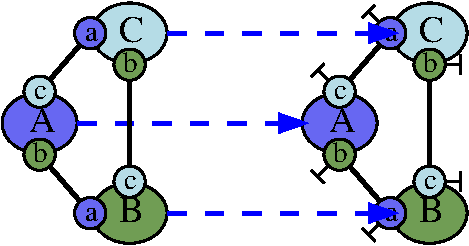
\includegraphics{generated_pictures/abc_embed.pdf}}\hfill\mbox{}
\caption{The unique morphism from the $\Sigma$-graph $\mathcal{T}_{\Sigma}$
and the $\Sigma$-graph $\mathcal{T}_{\textit{CM}}$.}
\label{fig:abc:embed}
\end{figure}
\begin{myexample}[morphisms (model of the triangle)]
  \renewcommand{\graphsymb}{\mathcal{T}}
A morphism between the $\Sigma$-graph $\graphsymb_{\Sigma}$ and the $\Sigma$-graph $\graphsymb_{\textit{CM}}$ is depicted in Fig.~\ref{fig:abc:embed}. This morphism maps any agent of the $\Sigma$-graph
$\graphsymb_{\Sigma}$ to the unique agent of the $\Sigma$-graph $\graphsymb_{\textit{CM}}$ having the same type.
This is indeed the unique morphism from the  $\Sigma$-graph
$\graphsymb_{\Sigma}$ to the $\Sigma$-graph $\graphsymb_{\textit{CM}}$.
\end{myexample}

\begin{figure}[t]
\hfill\scalebox{0.4}{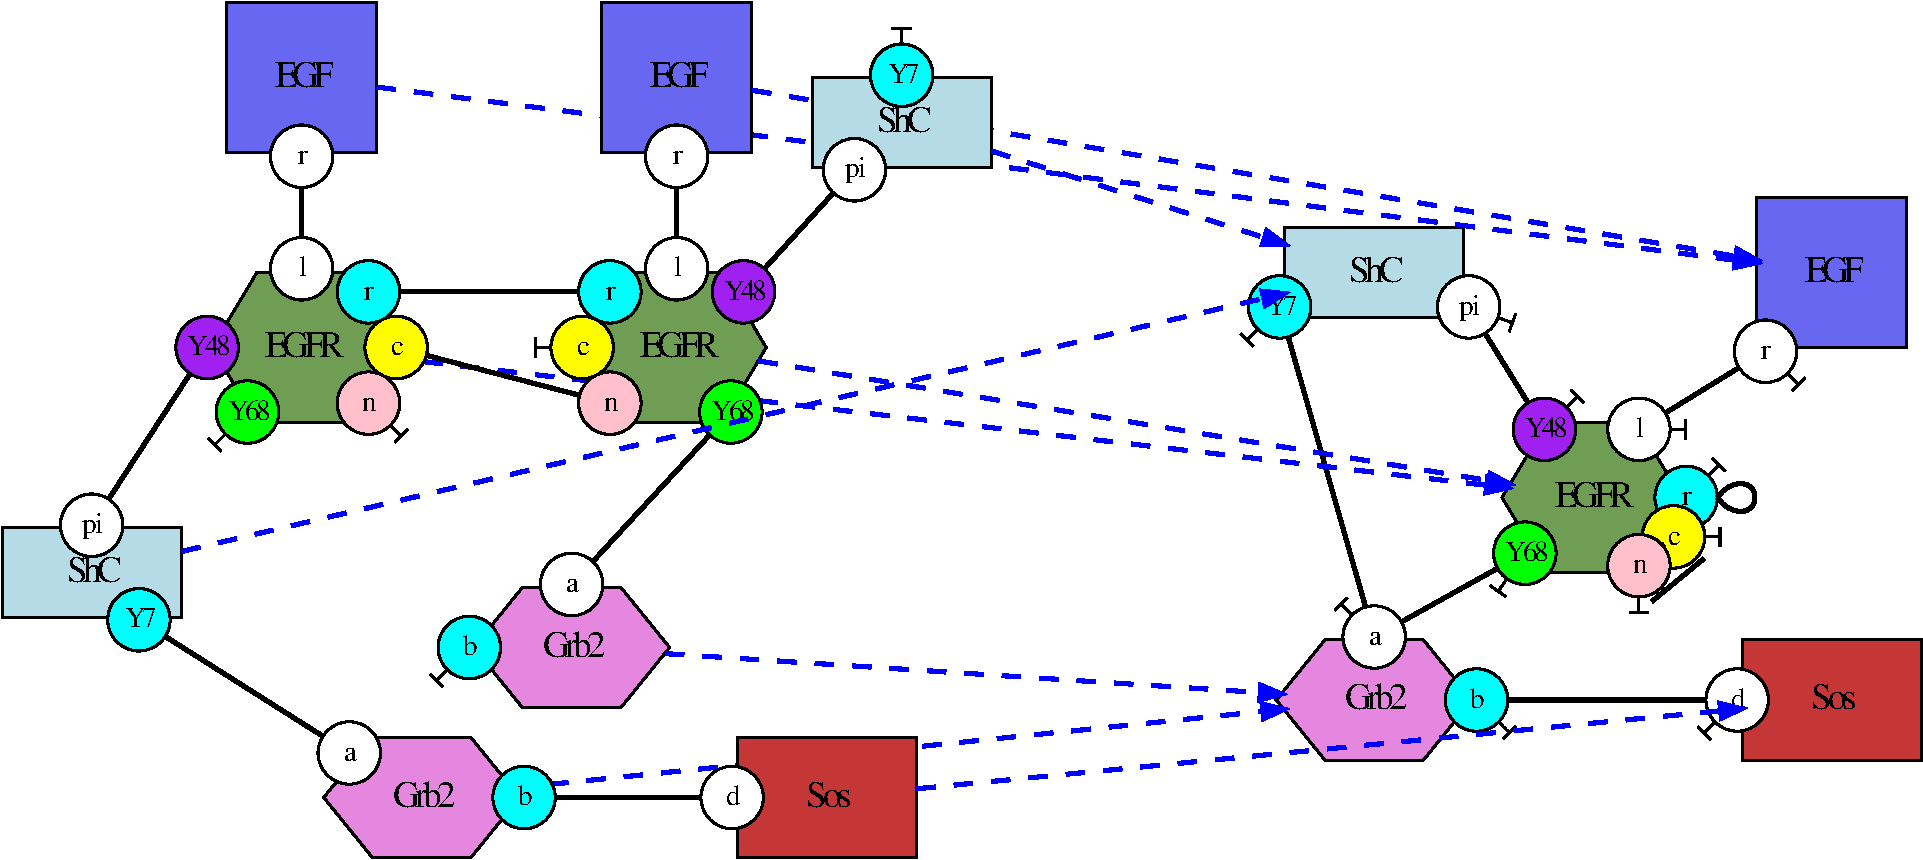
\includegraphics{generated_pictures/egfr_embed.pdf}}\hfill\mbox{}
\caption{The unique morphism from the $\Sigma$-graph $\graphsymb_{\Sigma}$
and the $\Sigma$-graph $\graphsymb_{\textit{CM}}$.}
  \label{fig:egfr:embed}
\end{figure}
\begin{myexample}[morphisms (EGF model)]

A morphism between the $\Sigma$-graph $\graphsymb_{\Sigma}$ and the $\Sigma$-graph $\graphsymb_{\textit{CM}}$ is depicted in Fig.~\ref{fig:egfr:embed}. This morphism maps any agent of the $\Sigma$-graph
$\graphsymb_{\Sigma}$ to the unique agent of the $\Sigma$-graph $\graphsymb_{\textit{CM}}$ having the same type.
This is indeed the unique morphism from the  $\Sigma$-graph
$\graphsymb_{\Sigma}$ to the $\Sigma$-graph $\graphsymb_{\textit{CM}}$.
\end{myexample}

%The following function: $[1 \mapsto 1, 2 \mapsto 1, 3\mapsto 2, 4\mapsto 3]$ induces a morphism from the $\Sigma$-graph $\graphsymb_{\Sigma}$ into the $\Sigma$-graph $\graphsymb_{\textit{CM}}$. This morphism is graphically described in Fig.~\ref{fig:morphism}. We notice that both agents of type \agentfont{A} have been merged into a single agent in the contact map, while merging the potential states of their sites. This way, the contact map
%provides a coarser
%(context-insensitive) summary of potential bonds in a model.
%\end{myexample}

Two morphisms from a $\Sigma$-graph  $E$ to a $\Sigma$-graph $F$, and from the $\Sigma$-graph $F$ to a $\Sigma$-graph $G$ respectively, compose in the usual way (and form a morphism from the $\Sigma$-graph $E$ into the
$\Sigma$-graph  $G$).

\subsection{Patterns and embeddings}

Now we restrict the definition of $\Sigma$-graphs so as to
focus on the ones that may express parts of the state of the system.
These $\Sigma$-graphs, that we call patterns, are defined as follows:

%\begin{figure}[t]
%
%\subfigure[The pattern $P$.]{%
%\label{fig:pattern}
%\begin{minipage}{\keep{\explainweakembedding}{0.3}{0.2}\linewidth}%
%\vspace*{16mm}\begin{center}
%  \scalebox{0.4}{\includegraphics{generated_pictures/pattern.pdf}}\vspace*{3mm}\vspace*{0.45cm}\smallskip\\%
%\end{center}
%\end{minipage}}
%\keep{\explainweakembedding}{\subfigure[The pattern $P'$.]{%
%\label{fig:patternbis}
%\begin{minipage}{0.3\linewidth}%
%\vspace*{8mm}\begin{center}
%  \scalebox{0.4}{\includegraphics{generated_pictures/patternprime.pdf}}
%  \vspace*{29.3mm}\smallskip\\%
%\end{center}
%\end{minipage}}}{}
%\subfigure[The bio-molecular compound $S$.]{%
%\label{fig:species}
%\begin{minipage}{0.3\linewidth}%
%  \vspace*{8mm}
%\begin{center}\scalebox{0.4}{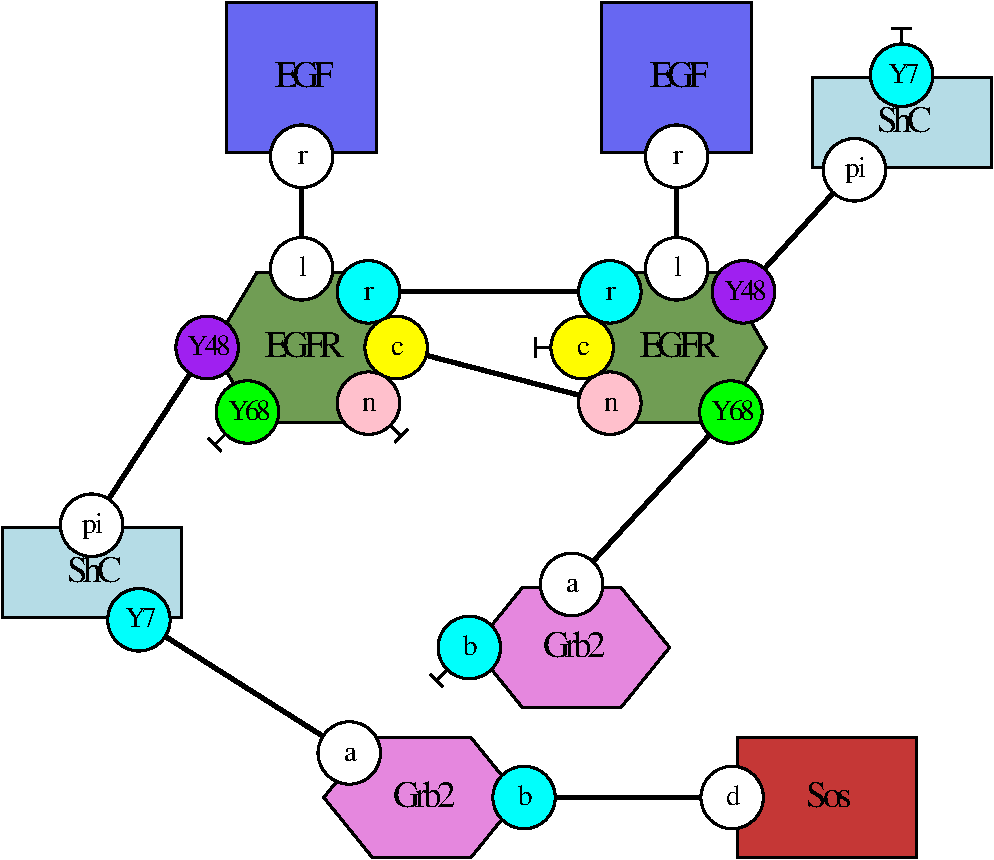
\includegraphics{generated_pictures/species.pdf}}\vspace*{3.8mm}\smallskip\\\end{center}%
%\end{minipage}}%
%\keep{\explainweakembedding}{
%
%}{}%
%\subfigure[An embedding from $P$ into $S$.]{%
%\label{fig:embedding}
%\begin{minipage}{0.45\linewidth}%
%\begin{center}%\scalebox{\keep{\explainweakembedding}{0.6}{0.6}}{\includegraphics{generated_pictures/embedding.pdf}}\smallskip\\
%  \end{center}%
%\end{minipage}}
%\keep{\explainweakembedding}{\subfigure[A weak emnbedding from $P'$ into $S'$.]{%
%\label{fig:weakembedding}
%\begin{minipage}{0.45\linewidth}
%  \begin{center}
%      \scalebox{\keep{\explainweakembedding}{0.6}{0.6}}{\includegraphics{generated_pictures/weak_embedding.pdf}}\smallskip\\
%  \end{center}
%\end{minipage}}}{}
%\caption{\keep{\explainweakembedding}{Three}{Two} patterns $P$\keep{\explainweakembedding}{, $P'$,}{} and $S$,  \keep{\explainweakembedding}{}{and} an embedding from the pattern $P$ to the bio-molecular compound $S$\keep{\explainweakembedding}{, and a weak embedding from the pattern $P'$ to the bio-molecular compound $S$}{}. \keep{\explainweakembedding}{There is no embedding from $P'$ to $S$.}{} The pattern $S$ is a species: it forms a connected component and the state of each site in  each agent is fully documented.}
%\label{fig:patterns}
%\end{figure}


\begin{defn}[patterns]
A pattern is a $\Sigma$-graph $P$ such that, for every site $s\in\sites[P]$ both following conditions are satisfied:
\begin{enumerate}
\item the set $\links[P](s)$ contains at most one element;
\item the set $\links[P](s)$ does not contain the element $s$.
\end{enumerate}
\end{defn}
The first condition ensures that the state of every site is either unspecified,
or free, or bound to a single specific site. The second condition ensures that a site is never bound to itself.


%\begin{myexample}[patterns]
%We give \keep{\explainweakembedding}{three}{two} examples of patterns. We consider the pattern $P%\bydef\graphtuple[P]$ that is defined as follows:
%\begin{enumerate}
%  \item $\agents[P]\bydef\{1\}$;
%  \item $\type[P]\bydef [1 \mapsto \agent{A}{}]$;
%  \item $\sites[P]\bydef\{(1,1),(1,3)\}$;
%  \item $\links[P]\bydef [(1,1)\mapsto \{\bound{}\}, (1,3)\mapsto \{\freesymbol{}\}]$\keep{\explainweakembedding}{,}{;}
%\end{enumerate}
%\keep{\explainweakembedding}{the pattern $P'%\bydef\graphtuple[P']$ that is defined as follows:
%\begin{enumerate}
%  \item $\agents[P']\bydef\{1\}$;
%  \item $\type[P']\bydef [1 \mapsto \agent{A}{}]$;
%  \item $\sites[P']\bydef\{(1,3)\}$;
%  \item $\links[P']\bydef [(1,3)\mapsto \{\freesymbol\}]$;
%\end{enumerate}}{}
%and the pattern $S%\bydef\graphtuple[S]
%$ that is defined as follows:
%\begin{enumerate}
%  \item $\agents[S]\bydef\{1,2,3,4\}$;
%  \item $\type[S]\bydef [1 \mapsto \agent{A}{}, 2 \mapsto \agent{A}{}, 3 \mapsto \agent{B}{}, 4 \mapsto \agent{C}{}]$;
%  \item $\sites[S]\bydef\left\{\begin{array}{l}(1,1),(1,2),(1,3),(2,1),(2,2),(2,3),\cr
%  (3,1),
%                               (3,2),(3,3),(3,4),(4,1),(4,2)\end{array}\right\}$;
%  \item $\links[S]\bydef
%\left[\begin{array}{l}
%      (1,1)\mapsto\{(3,1)\},
%      (1,2)\mapsto\{(3,2)\},
%      (1,3)\mapsto\{\freesymbol\},\cr
%      (2,1)\mapsto\{\freesymbol\},
%      (2,2)\mapsto\{(3,3)\},
%      (2,3)\mapsto\{\freesymbol\},\cr
%      (3,1)\mapsto\{(1,1)\},
%      (3,2)\mapsto\{(1,2)\},
%      (3,3)\mapsto\{(2,2)\},
%      (3,4)\mapsto\{(4,1)\},\cr
%      (4,1)\mapsto\{(3,4)\},
%      (4,2)\mapsto\{\freesymbol{}\}\end{array}\right]$.
%\end{enumerate}
%The patterns $P$\keep{\explainweakembedding}{, $P'$,}{} and $S$
%are graphically described respectively in Figs.~\ref{fig:pattern}\keep{\explainweakembedding}{,~\ref{fig:patternbis}}{}  and \ref{fig:species}.
%\end{myexample}


A bio-molecular compound is a connected pattern in which the state of each site is documented (no further information may be added).

Patterns may be related by embeddings. Besides preserving the structure of patterns, embeddings map agents to agents injectively.

\begin{defn}[embeddings]
  An embedding is a morphism from a pattern into another one, that is induced by an injective agent function.
\end{defn}

As opposed to classical notions of embeddings between graphs, embeddings between patterns preserve free sites.
When there exists an embedding from a pattern $E$ into a pattern $F$, we often write that the pattern $E$ embeds in the pattern $F$, or that $E$ occurs in the pattern $F$. The composition of two embeddings is an embedding. Two patterns $E$ and $F$ are isomorphic whenever there exist an embedding from the pattern $E$ to the pattern $F$ and an embedding from the pattern $F$ to the pattern $E$, which is denoted as $E \iso F$.  We also denote as $[E]_{\iso}$ the $\iso$-equivalence class of the pattern $E$. The $\iso$-equivalence class $[E]_{\iso}$ of the pattern $E$ is made of all the patterns that are isomorphic to the pattern $E$.

\section{Reasoning on repeatable patterns}
\label{sec:graphs}

In this section, we formalise the problem of deciding whether or not a contact map is compatible with an infinite set of bio-molecular compounds. Then we introduce two kinds of graph to reason about this problem.

\subsection{Interpretation of a contact map}

Intuitively, a contact map may be interpreted as the set of the bio-molecular compounds which may be projected into that contact map by the means of a morphism. However this notion is not relevant to reason about the finiteness of the set of the bio-molecular compounds in  a given model. Indeed with such a  definition,  each model admitting at least one bio-molecular compound would admit an infinite number of bio-molecular compounds due to isomorphisms. Thus we consider $\iso$-equivalence classes of bio-molecular compounds instead.


\begin{defn}[interpretation of a contact map]
The interpretation $\llbracket \graphsymb_{\textit{CM}} \rrbracket$ of a contact map $\graphsymb_{\textit{CM}}$ is defined as the set of all the $\iso$-equivalence classes of bio-molecular compound $[G]_{\iso}$ such that there exists a morphism from the site graph $G$ into the contact map $\graphsymb_{\textit{CM}}$.
\end{defn}

We can now state properly the problem we want to solve:
\begin{problem}\label{problem}
Let $\graphsymb_{\textit{CM}}$ be a contact map.
We are looking for an automatic prodecure to decide whether
the set $\llbracket \graphsymb_{\textit{CM}} \rrbracket$ is finite, or not.
\end{problem}

\subsection{Chains}

In this section, we introduce a kind of pumping lemma in order to reduce
Problem \ref{problem} to the one of detecting a repeatable pattern.

Firstly, we define properly a repeatable pattern as a chain of agents which may be iterated to form arbitrarily long patterns.

\begin{defn}[Chain]
A pattern is called a chain if and only if it satisfies the following properties:
\begin{enumerate}
  \item every agent documents at most two sites;
  \item there is an agent with a site free or
  that documents at most one site (or both);
  \item at most two agents do not have two sites bound.
\end{enumerate}
\end{defn}

In particular, every chain is connected.
A chain is formed either of a single agent with at most two sites all free, or of a linear chain of agents with exactly two extremities. In the latter case, every agent not in the extremities has two sites and these sites are bound. The agents on the extremity either have exactly one site that is bound. Additionally, it may have at most one other site (which is free).

A chain is a repeatable patterns whenever it contains at least two agents and its extremities may be replug to each other. This is formalised as follows.

\begin{defn}[repeatable pattern]
A chain is called a repeatable pattern if and only if the following conditions are satisfied:
\begin{enumerate}
\item it has two distinct extremities;
\item it has no free sites;
\item both agents at the extremities are of the same kind;
\item both sites documented at the extremities are different.
\end{enumerate}
A repeatable pattern is said elementary if and only if it contains no occurrence of repeatable patterns (besides itself).
\end{defn}

\begin{figure}[t]
\subfigure[A chain with one site free.]{%
\begin{minipage}{0.45\linewidth}
\label{fig:repeatable:a}
\centering\scalebox{0.6}{
\includegraphics{generated_pictures/abc_pattern_a.pdf}}
\end{minipage}}%
\subfigure[A chain with two extremities of different kinds.]{%
\begin{minipage}{0.45\linewidth}
\label{fig:repeatable:b}
\centering\scalebox{0.6}{
\includegraphics{generated_pictures/abc_pattern_b.pdf}}
\end{minipage}}%

\subfigure[A chain with two extremities documenting the same site.]{%
\begin{minipage}{0.45\linewidth}
\centering\scalebox{0.4}{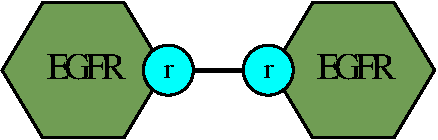
\includegraphics{generated_pictures/egfr_egfr_r.pdf}}
\label{fig:repeatable:c}
\end{minipage}}%
\subfigure[An elementary repeatable pattern.]{%
\begin{minipage}{0.45\linewidth}
\label{fig:repeatable:d}
\centering\scalebox{0.6}{
\includegraphics{generated_pictures/abc_pattern.pdf}}
\end{minipage}}
\caption{Four patterns. Each of them is a chain. But only the last one is repeatable.}
\label{fig:repeatable}
\end{figure}

\begin{exmp}
  We consider four patterns in Fig.~\ref{fig:repeatable}.
  All these patterns are chains.
  The pattern in Fig.~\ref{fig:repeatable:a} is not repeatable because one of its extremity has a free site.
  The pattern in Fig.~\ref{fig:repeatable:b} is not repeatable
  because its extremities are not of the same kind.
  The pattern in Fig.~\ref{fig:repeatable:c} is not repeatable
  because its extremities document the same site
  The pattern in Fig.~\ref{fig:repeatable:d} is repeatble (and elementary).
\end{exmp}

We can now establish our pumping lemma.
\begin{lemma}[pumping lemma]
Let $\graphsymb_{\textit{CM}}$ be a contact map.
Both following assertions are equivalent:
\begin{enumerate}
  \item The set $\llbracket \graphsymb_{\textit{CM}} \rrbracket$ is infinite;
  \item There exist an elementary repeatable pattern $P$ and a morphism
  between the pattern $P$ and the contact map $\graphsymb_{\textit{CM}}$.
\end{enumerate}
\end{lemma}

\subsection{Graph of the sites}

It is  tempting to interpret the following repeatable pattern:
\begin{equation*}
\scalebox{0.6}{
\includegraphics{generated_pictures/abc_pattern.pdf}}
\end{equation*}
as the sequence of sites $\sitefont{b}$ of $\agentfont{A}$, $\sitefont{a}$ of $\agentfont{B}$, $\sitefont{c}$ of $\agentfont{B}$, $\sitefont{b}$ of $\agentfont{C}$, $\sitefont{a}$ of $\agentfont{C}$, and $\sitefont{c}$ of $\agentfont{A}$. Yet in this sequence, sites are polarised.
Each site on a odd position and the next one always belong to the same kind of protein.
While there always exists a link between each site on an even position and the next one. Due to this polarisation, it is tempting to consider the sub-sequence of each other site in that sequence of sites.

Next we define a graph that stands for all the potential sequences of sites that may occur on even occurrences in the repeatable patterns that are compatible with a given contact map. This is the graph of the sites of this contact map.

\begin{defn}[graph of the sites]
  Let $\graphsymb_{\textit{CM}}$ be a contact map.

  The contact map $\graphsymb_{\textit{CM}}$ is associated with a classical graph $(\mathcal{V},\mathcal{E})$, called the graph of the sites of the contact map $\graphsymb_{\textit{CM}}$, which is defined as follows:
  \begin{itemize}
    \item $\mathcal{V}$ is the set $\sites[\graphsymb_{\textit{CM}}]$ of the sites of the $\Sigma$-graph $\graphsymb_{\textit{CM}}$.
    \item $\mathcal{E}$ is the subset of $V\times V$ such that
    $((n,i),(n',i'))\in E$ if and only if there exists a site
    $i''\in\linksite(\type[\graphsymb_{\textit{CM}}](n'))$ such that:
    $i'' \neq i'$ and $(n',i'')\in\links[\graphsymb_{\textit{CM}}](n,i)$.
  \end{itemize}
  \end{defn}

In the edges of the graph of the sites, the sites via with we enter the target agent is kept implicit.

The following theorem relates the cycles in the graph of the sites to the existence of repeatable patterns.

\begin{theorem}
  \label{th:site}
  Let $\graphsymb_{\textit{CM}}$ be a contact map.

Let $\agentfont{A}$ and $\agentfont{B}$ be two kinds of agent and
$i$ and $i'$ be two site names.

  Both following properties are equivalent:
  \begin{enumerate}
    \item There exists a repeatable pattern
    with an agent of kind $\agentfont{A}$ connected via its site $i$
    to one site of an agent of kind $\agentfont{B}$ itself connected to another agent on site $i'$.
\item There exist two agents $n$ and $n'$ respectively of kinds $\agentfont{A}$
and  $\agentfont{B}$, and a  cycle in the graph of the sites of the contact map    $\graphsymb_{\textit{CM}}$  that passes by the edge $((n,i),(n',i'))$.
  \end{enumerate}
\end{theorem}

Thus, Thm.~\ref{th:site} reduces the problem of deciding whether
a contact map is compatible with an infinite number of non-isomorphic bio-molecular compounds to the one of computing the strongly connected components of the graph of the sites of this contact map.

\begin{figure}
  \subfigure[Contact map.]%
  {\begin{minipage}{0.4\linewidth}\label{fig:abc:gs:cm}\centering\scalebox{0.4}{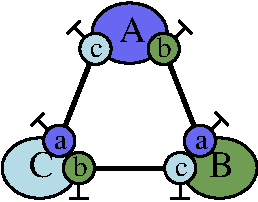
\includegraphics{generated_pictures/abc_contact_map.pdf}}\end{minipage}}%
  \subfigure[Graph of the sites.]%
  {\begin{minipage}{0.59\linewidth}\label{fig:abc:gs:gs}
  \xymatrix@C=0.cm@R=0.35cm{
  \begin{minipage}{0.6cm}
  \scalebox{0.35}{
\includegraphics{generated_pictures/a_b.pdf}}
  \end{minipage}
  \ar@{->}[rr]
  &&
  \begin{minipage}{0.6cm}
  \scalebox{0.35}{
\includegraphics{generated_pictures/b_c.pdf}}
  \end{minipage}
  \ar@{->}[ld]
  &&&
  \begin{minipage}{0.6cm}
  \scalebox{0.35}{
\includegraphics{generated_pictures/c_b.pdf}}
  \end{minipage}
  \ar@{->}[rd]
  \cr
&
\begin{minipage}{0.6cm}
\scalebox{0.35}{
\includegraphics{generated_pictures/c_a.pdf}}
\end{minipage}
\ar@{->}[lu]
&&&
\begin{minipage}{0.6cm}
\scalebox{0.35}{
\includegraphics{generated_pictures/a_c.pdf}}
\end{minipage}
\ar@{->}[ru]
&&
\begin{minipage}{0.6cm}
\scalebox{0.35}{
\includegraphics{generated_pictures/b_a.pdf}}
\end{minipage}
\ar@{->}[ll]
 }\end{minipage}}

  \caption{ABC model. In \ref{fig:abc:gs:cm}, we recall the contact map.
  In Fig.~\ref{fig:abc:gs:gs}, we give the graph of the sites that is associated with this contact map. The nodes of these graphs are the sites of the contact map. There is an oriented edge between a node $s$ and a node $t$ if and only if there is a site connected in the contact map to the site $s$, in the same kind of protein as the site $t$ but distinct from $t$. }
  \label{fig:abc:gs}
\end{figure}


\begin{figure}
  \subfigure[Contact map.]%
  {\begin{minipage}{0.4\linewidth}\label{fig:egfr:gs:cm}\scalebox{0.4}{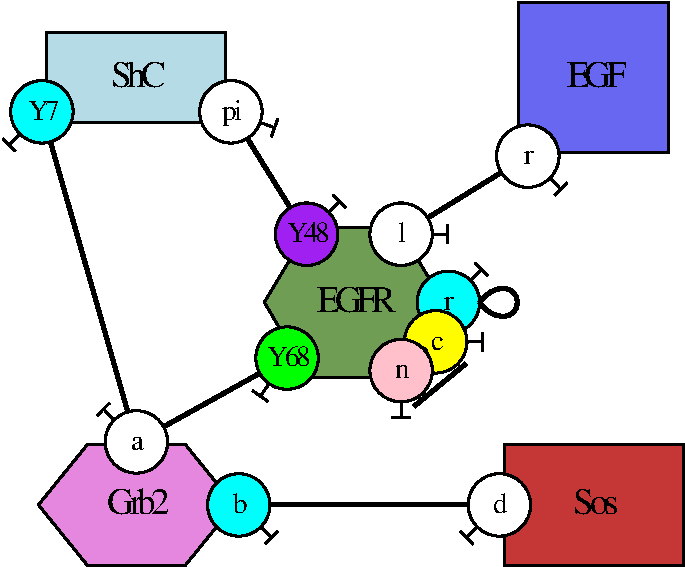
\includegraphics{generated_pictures/contact_map.pdf}}\end{minipage}}%
  \subfigure[Graph of the sites.]%
  {\begin{minipage}{0.59\linewidth}\label{fig:egfr:gs:gs}
  \xymatrix@C=0.cm@R=0.35cm{
  &&&\begin{minipage}{1cm}
  \scalebox{0.35}{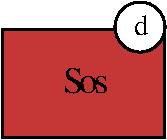
\includegraphics{generated_pictures/sos_d.pdf}}
  \end{minipage}
  \ar@{->}[d]&&&&\cr
  &
  \begin{minipage}{1cm}\scalebox{0.35}{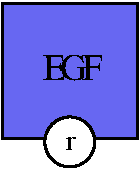
\includegraphics{generated_pictures/egf_r.pdf}}\end{minipage}
    \ar@{->}[dl]
    \ar@{->}[drrr]
    \ar@{->}[ddrrrr]
    \ar@{->}@/_{0.6cm}/[ddrr]
    \ar@{->}[dr]
    &&
  \begin{minipage}{1cm}\scalebox{0.35}{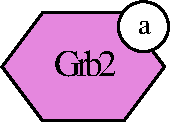
\includegraphics{generated_pictures/grb2_a.pdf}}\end{minipage}
    \ar@{->}[rr]
    \ar@{->}[dlll]
    \ar@{->}[dl]
    \ar@{->}[dr]
    \ar@{->}[dd]
    \ar@{->}@/_{0.6cm}/[ddll]&&
  \begin{minipage}{1cm}
    \scalebox{0.35}{
\includegraphics{generated_pictures/shc_pi.pdf}}
    \end{minipage}
    \ar@{->}[dlllll]
    \ar@{->}[dlll]
    \ar@{->}[dl]
    \ar@{->}[dd]
    \ar@{->}[ddllll]\cr
  \begin{minipage}{1cm}\scalebox{0.35}{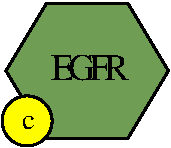
\includegraphics{generated_pictures/egfr_c.pdf}}\end{minipage}
    \ar@{->}[rr]
    \ar@{->}[dr]
    \ar@{->}[drrr]
    \ar@{->}[drrrrr]
    \ar@{->}@(ul,dl)
    &&
  \begin{minipage}{1cm}\scalebox{0.35}{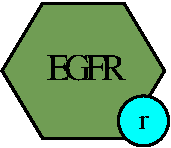
\includegraphics{generated_pictures/egfr_r.pdf}}\end{minipage}
    \ar@{->}[ll]
    \ar@{->}[dl]
    \ar@{->}[dr]
    \ar@{->}[drrr]
    \ar@{->}[rr]&&
  \begin{minipage}{1cm}\scalebox{0.35}{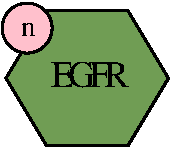
\includegraphics{generated_pictures/egfr_n.pdf}}\end{minipage}
    \ar@{->}[ll]
    \ar@{->}[dl]
    \ar@{->}[dlll]
    \ar@{->}[dr]
    \ar@{->}@(ur,dr)&&\cr
  &
  \begin{minipage}{1cm}\scalebox{0.35}{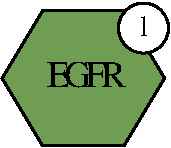
\includegraphics{generated_pictures/egfr_l.pdf}}\end{minipage}&&
  \begin{minipage}{1cm}\scalebox{0.35}{\includegraphics{generated_pictures/egfr_Y48.pdf}}\end{minipage}\ar@{->}[d]&&
  \begin{minipage}{1cm}\scalebox{0.35}{\includegraphics{generated_pictures/egfr_Y68.pdf}}\end{minipage}\ar@{->}[d]\cr
  &&&
  \begin{minipage}{1cm}\scalebox{0.35}{\includegraphics{generated_pictures/shc_Y7.pdf}}\ar@{->}[rr]\end{minipage}
  &&\begin{minipage}{1cm}\scalebox{0.35}{\includegraphics{generated_pictures/grb2_b.pdf}}\end{minipage}&&\cr }\end{minipage}}

  \caption{EGF model. In \ref{fig:egfr:gs:cm}, we recall the contact map.
  In Fig.~\ref{fig:egfr:gs:gs}, we give the graph of the sites that is associated with this contact map.  }
  \label{fig:egfr:gs}
\end{figure}

\begin{exmp}[graph of the sites (ABC model)]
In Fig.~\ref{fig:abc:gs}, we compute the graph of the sites for the contact map of the model with three proteins that may form a triangle. It is worth noticing that this graph is made of exactly two non trivial strongly connected components.
Each one corresponds to the triangle \agentfont{ABC} depending whether it is scanned clockwise or counter-clockwise. Further constraints would be required on the bio-molecular compounds of the models to prove that there is a finite amount of them (the contact map of the model is compatible with an infinite number of them).
\end{exmp}

\begin{exmp}[graph of the sites (EGF model)]
In Fig.~\ref{fig:egfr:gs}, we compute the graph of the sites for the contact map of the model of the early events in the integration of the epidermic growth factor. It is worth noticing that this graph has only the following non trivial strongly connected component:
\begin{equation*}\hspace*{1cm}\scalebox{1.5}{\xymatrix@C=0.5cm@R=0.35cm{\begin{minipage}{1cm}\scalebox{0.3}{\includegraphics{generated_pictures/egfr_c.pdf}}\end{minipage}
  \ar@{->}[rr]
  \ar@{->}@(ul,dl)
  &&
\begin{minipage}{1cm}\scalebox{0.3}{\includegraphics{generated_pictures/egfr_r.pdf}}\end{minipage}
  \ar@{->}[ll]
  \ar@{->}[rr]&&
\begin{minipage}{1cm}\scalebox{0.3}{\includegraphics{generated_pictures/egfr_n.pdf}}\end{minipage}
  \ar@{->}[ll]
  \ar@{->}@(ur,dr)&&}}\end{equation*}
Further constraints are required on the bio-molecular compounds of the models to prove that there is a finite amount of them (the contact map of the model is compatible with an infinite number of different bio-molecular compounds).
\end{exmp}


\subsection{Graph of the potential links}

We do not know how to refine the graph of the sites of a given contact map to take into account further constraints about the reachable bio-molecular compounds. We consider in this section another kind of graphs which focuses on the different links in the contact map and that will be easier to refine.

Now we interpret the following repeatable pattern:
\begin{equation*}
\scalebox{0.6}{\includegraphics{generated_pictures/abc_pattern.pdf}}
\end{equation*}
as the sequence of (oriented) links from the
site $\sitefont{b}$ of $\agentfont{A}$ to the site
 $\sitefont{a}$ of $\agentfont{B}$,
 %from the site $\sitefont{a}$ of $\agentfont{B}$ to the site $\sitefont{c}$ of $\agentfont{B}$,
 from the site $\sitefont{c}$ of $\agentfont{B}$ to the site $\sitefont{b}$ of $\agentfont{C}$,
 %from the site $\sitefont{b}$ of $\agentfont{C}$ to the site $\sitefont{a}$ of $\agentfont{C}$,
 and from the site $\sitefont{a}$ of $\agentfont{C}$ to the site $\sitefont{c}$ of $\agentfont{A}$.

In the following, we define a graph that stands for all the potential sequences of links that may occur on repeatable patterns that are compatible with a given contact map. We call this graph the graph of the potential links.

\begin{defn}[graph of the potential links]
  Let $\graphsymb_{\textit{CM}}$ be a contact map.

  The contact map $\graphsymb_{\textit{CM}}$ is associated with a classical graph $(\mathcal{V},\mathcal{E})$, called the graph of the sites that is defined as follows:
  \begin{itemize}
    \item $\mathcal{V}$ is the subset of the pairs of elements $(s,s')$ of the set  $\sites[\graphsymb_{\textit{CM}}]$ of the sites of the $\Sigma$-graph $\graphsymb_{\textit{CM}}$ such that $s'=\links[\graphsymb_{\textit{CM}}](s)$.
    \item $\mathcal{E}$ is the subset of the pairs $((s,s'),(s'',s'''))$ of pairs of sites in $\mathcal{V}\times\mathcal{V}$ for which  there exists an agent $n\in\agents[\graphsymb_{\textit{CM}}]$ and two different site names $i$ and $i' \in\linksite(\type[\graphsymb_{\textit{CM}}])$ such that $s'=(n,i)$ and $s''=(n,i')$.
  \end{itemize}
  \end{defn}

The condition on the edges of the graph of the potential links ensures that
both links may be consecutive in a repeatable pattern.

The following theorem relates the cycles in the graph of the potential links to the existence of repeatable patterns.

\begin{theorem}
  \label{th:links}
  Let $\graphsymb_{\textit{CM}}$ be a contact map.

Let $\agentfont{A}$ and $\agentfont{B}$ be two kinds of agent and
$i$ and $i'$ be two site names.

  Both following properties are equivalent:
  \begin{enumerate}
    \item There exists a repeatable pattern
    with an agent of kind $\agentfont{A}$ connected via its site $i$
    to the site $i'$ of an agent of kind $\agentfont{B}$;
\item There exist two agents $n$ and $n'$ respectively of kinds $\agentfont{A}$
and  $\agentfont{B}$, and a  cycle in the graph of the potential links of the contact map    $\graphsymb_{\textit{CM}}$  that passes by the vertex $((n,i),(n',i'))$.
  \end{enumerate}
\end{theorem}

Thus, Thm.~\ref{th:links} reduces the problem of deciding whether
a contact map is compatible with an infinite number of non-isomorphic bio-molecular compounds to the one of computing the strongly connected components of the graph of its potential links.


\begin{figure}
  \subfigure[Contact map.]%
  {\begin{minipage}{0.4\linewidth}\label{fig:abc:gl:cm}\centering\scalebox{0.4}{\includegraphics{generated_pictures/abc_contact_map.pdf}}\end{minipage}}%
  \subfigure[Graph of the potential successive links.]%
  {\begin{minipage}{0.59\linewidth}\label{fig:abc:gl:gl}
  \xymatrix@C=0.cm@R=0.35cm{
  \begin{minipage}{1.2cm}
  \scalebox{0.35}{\includegraphics{generated_pictures/link_a_b.pdf}}
  \end{minipage}
  \ar@{->}[rr]
  &&
  \begin{minipage}{1.2cm}
  \scalebox{0.35}{\includegraphics{generated_pictures/link_b_c.pdf}}
  \end{minipage}
  \ar@{->}[ld]
  &&&
  \begin{minipage}{1.2cm}
  \scalebox{0.35}{\includegraphics{generated_pictures/link_c_b.pdf}}
  \end{minipage}
  \ar@{->}[rd]
  \cr
&
\begin{minipage}{1.2cm}
\scalebox{0.35}{\includegraphics{generated_pictures/link_c_a.pdf}}
\end{minipage}
\ar@{->}[lu]
&&&
\begin{minipage}{1.2cm}
\scalebox{0.35}{\includegraphics{generated_pictures/link_a_c.pdf}}
\end{minipage}
\ar@{->}[ru]
&&
\begin{minipage}{1.2cm}
\scalebox{0.35}{\includegraphics{generated_pictures/link_b_a.pdf}}
\end{minipage}
\ar@{->}[ll]
 }\end{minipage}}
 \caption{ABC model. In \ref{fig:abc:gl:cm}, we recall the contact map.
 In Fig.~\ref{fig:abc:gl:gl}, we give the graph of the links that is associated with this contact map. The nodes of these graphs are obtained by orienting the links of the contact map (hence there are two nodes per links). }
  \label{fig:abc:gl}
\end{figure}


\newcommand{\minipagesize}{1.3cm}
\newcommand{\factor}{0.15}
\begin{figure}
  \subfigure[Contact map.]%
  {\begin{minipage}{0.4\linewidth}\label{fig:egfr:gl:cm}\scalebox{0.4}{\includegraphics{generated_pictures/contact_map.pdf}}\end{minipage}}%
  \subfigure[Graph of the potential links.]%
  {%
  \begin{minipage}{0.59\linewidth}\label{fig:egfr:gl:gl}
  \xymatrix@C=0.cm@R=0.35cm{
  &&&
  \begin{minipage}{\minipagesize}\scalebox{\factor}{\includegraphics{generated_pictures/sos_grb2.pdf}}\end{minipage}
  \ar@{->}[rr]
  \ar@{->}[d]&&
  \begin{minipage}{\minipagesize}\scalebox{\factor}{\includegraphics{generated_pictures/grb2_shc.pdf}}\end{minipage}
    \ar@{->}[d]
  &&\cr
  &
  \begin{minipage}{\minipagesize}\scalebox{\factor}{\includegraphics{generated_pictures/egf_egfr.pdf}}\end{minipage}
    \ar@{->}[dl]
    \ar@{->}[drrr]
    \ar@{->}[ddrrrr]
    \ar@{->}@/_{0.6cm}/[ddrr]
    \ar@{->}[dr]
    &&
  \begin{minipage}{\minipagesize}\scalebox{\factor}{\includegraphics{generated_pictures/grb2_egfr.pdf}}\end{minipage}
    \ar@{->}[dlll]
    \ar@{->}[dl]
    \ar@{->}[dr]
    \ar@{->}[dd]
    \ar@{->}@/_{0.6cm}/[ddll]&&
  \begin{minipage}{\minipagesize}\scalebox{\factor}{\includegraphics{generated_pictures/shc_egfr.pdf}}\end{minipage}
    \ar@{->}[dlllll]
    \ar@{->}[dlll]
    \ar@{->}[dl]
    \ar@{->}[dd]
    \ar@{->}[ddllll]\cr%
\begin{minipage}{\minipagesize}\hspace*{0.2cm}\scalebox{\factor}{\includegraphics{generated_pictures/egfr_egfr_c.pdf}}
\end{minipage}
    \ar@{->}[rr]
    \ar@{->}[dr]
    \ar@{->}[drrr]
    \ar@{->}[drrrrr]
    \ar@{->}@(ul,dl)
    &&
  \begin{minipage}{\minipagesize}\scalebox{\factor}{\includegraphics{generated_pictures/egfr_egfr_r.pdf}}\end{minipage}
    \ar@{->}[ll]
    \ar@{->}[dl]
    \ar@{->}[dr]
    \ar@{->}[drrr]
    \ar@{->}[rr]&&
  \begin{minipage}{\minipagesize}
    \scalebox{\factor}{\includegraphics{generated_pictures/egfr_egfr_n.pdf}}
  \end{minipage}
    \ar@{->}[ll]
    \ar@{->}[dl]
    \ar@{->}[dlll]
    \ar@{->}[dr]
    \ar@{->}@(ur,dr)&&\cr
  &
  \begin{minipage}{\minipagesize}\scalebox{\factor}{\includegraphics{generated_pictures/egfr_egf.pdf}}\end{minipage}
  &&
  \begin{minipage}{\minipagesize}\scalebox{\factor}{\includegraphics{generated_pictures/egfr_shc.pdf}}\end{minipage}
  \ar@{->}[d]&&
  \begin{minipage}{\minipagesize}\scalebox{\factor}{\includegraphics{generated_pictures/egfr_grb2.pdf}}\end{minipage}
  \ar@{->}[d]\cr
  &&&
  \begin{minipage}{\minipagesize}\scalebox{\factor}{\includegraphics{generated_pictures/shc_grb2.pdf}}\ar@{->}[rr]\end{minipage}
  &&
  \begin{minipage}{\minipagesize}\scalebox{\factor}{\includegraphics{generated_pictures/grb2_sos.pdf}}\end{minipage}
  &&\cr
    }
\end{minipage}}
  %\scalebox{0.4}{\includegraphics{generated_pictures/egfr_graph_site.pdf}}}
  \caption{EGF model. In \ref{fig:egfr:gl:cm}, we recall the contact map.
  In Fig.~\ref{fig:egfr:gl:gl}, we give the graph of the links that is associated with this contact map. There are two nodes per links, except for the link between the site $r$ of $EGFR$ and itself, for which there is a unique node.
  }
  \label{fig:egfr:gl}
\end{figure}


\begin{exmp}[graph of the potential links (ABC model)]
In Fig.~\ref{fig:abc:gl}, we compute the graph of the potential links for the contact map of the model with three proteins that may form a triangle. It is worth noticing that this graph is made of exactly two non trivial strongly connected components.
Each one corresponds to the triangle \agentfont{ABC} depending whether it is scanned clockwise or counter-clockwise. Further constraints would be required on the bio-molecular compounds of the models to prove that there is a finite amount of them (the contact map of the model is compatible with an infinite number of them).
\end{exmp}

\begin{exmp}[graph of the potential links (EGF model)]
In Fig.~\ref{fig:egfr:gl}, we compute the graph of the potential links for the contact map of the model of the early events in the integration of the epidermic growth factor. It is worth noticing that this graph has only one non trivial strongly connected component:
\begin{equation*}\hspace*{1cm}\scalebox{1.5}{\xymatrix@C=0.2cm@R=0.35cm{\begin{minipage}{1.2cm}\scalebox{0.15}{\includegraphics{generated_pictures/egfr_egfr_c.pdf}}\end{minipage}
  \ar@{->}[rr]
  \ar@{->}@(ul,dl)
  &&
\begin{minipage}{1.2cm}\scalebox{0.15}{\includegraphics{generated_pictures/egfr_egfr_r.pdf}}\end{minipage}
  \ar@{->}[ll]
  \ar@{->}[rr]&&
\begin{minipage}{1.5cm}\scalebox{0.15}{\includegraphics{generated_pictures/egfr_egfr_n.pdf}}\end{minipage}
  \ar@{->}[ll]
  \ar@{->}@(ur,dr)&&}}\end{equation*}
Further constraints are required on the bio-molecular compounds of the models to prove that there is a finite amount of them (the contact map of the model is compatible with an infinite number of them).
\end{exmp}

\section{Taking into account the result of a static analysis}

In this section, we explain how to refine the graph of the potential links of a given contact map, in order to take into some additional constraints about the potentially reachable bio-molecular compounds.
These constraints may come from a static analysis \cite{SASB2016,KaSa} taken as a black box and they may take the form of a set of patterns that shall occur in no reachable bio-molecular compounds.
These constraints cannot be written in the contact map which can cope only with non relational information about the potential state of sites.

In the case of the model of the early events of the integration of the epidermic growth factor, the analysis that is described in \cite{SASB2016} can infer automatically, from the set of rules and the initial state, that the following patterns:
\begin{equation*}
\scalebox{0.3}{\includegraphics{generated_pictures/egfr_r_c.pdf}}\hspace*{1cm} \scalebox{0.3}{\includegraphics{generated_pictures/egfr_r_n.pdf}}\hspace*{1cm} \scalebox{0.3}{\includegraphics{generated_pictures/egfr_n_c.pdf}}
\end{equation*}
are not reachable. That is to say that a receptor cannot be bound to two different other instances of receptors.


The analysis that is described in \cite{afp} generalises this approach to arbitrary cycles of proteins. In the example of the triangle, it infers (providing that it is a consequence of the rules and of the initial state), that no two \agentfont{A}s may occur in a given connected compound, by proving that the following pattern:
\begin{equation*}
\scalebox{0.6}{\includegraphics{generated_pictures/abc_pattern.pdf}}
\end{equation*}
is unreachable.

We refine the statement of Problem \ref{problem} so as take into account the constraints potentially coming from an external static analysis.


\begin{defn}[interpretation  with a set of forbidden patterns]
The interpretation $\llbracket \graphsymb_{\textit{CM}}, \mathcal{P}\rrbracket$ of a contact map $\graphsymb_{\textit{CM}}$ with a set of forbidden patterns $\mathcal{P}$ is defined as the set of the $\iso$-equivalence classes of bio-molecular compound $[G]_{\iso}$ such that there exists a morphism from the site graph $G$ into the contact map $\graphsymb_{\textit{CM}}$ and that $G$ contains no occurrence of patterns from the set $\mathcal{P}$.
\end{defn}
\begin{problem}\label{problembis}
Let $\graphsymb_{\textit{CM}}$ be a contact map and $\mathcal{P}$ be a set of patterns.

We are looking for an automatic procedure to decide whether
the set $\llbracket \graphsymb_{\textit{CM}},\mathcal{P} \rrbracket$ is finite, or not.
\end{problem}

In the following, we propose a graph structure to answer to Problem \ref{problembis}. Our approach is sound but not complete. It can detect and prove that the set of bio-molecular compounds is finite. But when it warns about potential repeatable patterns, it may be a false positive. We do not look for a complete procedure because on the first hand detecting whether or not a pattern is reachable is not decidable in Kappa \cite{kreyBig}, and on the second hand detecting whether a pattern may occur in a set of bio-molecular compounds that do not contain patterns from a given set is not so easy due to potential overlaps between patterns. Thus we rely on a sound but not complete procedure.

The main idea is to refine the graph of the potential successive links by labelling each edge with the pattern that is formed by fusing the source and the target of this edge.

The label of an edge must be understood as contextual information about the occurrence of two successive links. In order to take into account unreachable patterns, we introduce two operations to update refinements of the graph of the potential successive links. The first operation replace
an edge by several edges by refining its patterns into longer chains.
More precisely, given an edge, one shall decide which extremity of its label to refine and which site to insert, the former edge is potentially replaced by several ones, one for each potential partner of this site in the contact map. There may be several possibilities in case of competition on a binding site. The second operation consists in removing edges the label of which contain an occurrence of a forbidden pattern.


\begin{exmp}[graph refinement (the model of the triangle)]
  For instance the following edge
  \begin{equation*}\xymatrix@C=0.5cm@R=0.35cm{
  \begin{minipage}{1.2cm}
  \scalebox{0.35}{\includegraphics{generated_pictures/link_a_b.pdf}}
  \end{minipage}
  \ar@{->}[rr]
  &&
  \begin{minipage}{1.2cm}
  \scalebox{0.35}{\includegraphics{generated_pictures/link_b_c.pdf}}
  \end{minipage}}
  \end{equation*}
  will be labelled with the following pattern:
  \begin{equation*}
    \scalebox{0.35}{\includegraphics{generated_pictures/link_a_b_c.pdf}}.
  \end{equation*}

  This pattern may then be refined.
  We choose to refine the state of the site \sitefont{a} of the protein \agentfont{C}{}. This site has only one bond in the contact map, thus there is only the following possibility:
  \begin{equation}
      \scalebox{0.35}{\includegraphics{generated_pictures/abc_pattern.pdf}}.
  \end{equation}
  Yet this chain contains a black-listed pattern, thus the edge may be safely discarded from the graph.

  We obtain the graph that is depicted in Fig.~\ref{fig:abc:gll:gl}.
\end{exmp}

The following theorem states the soundness of our approach.
%It uses the notion of circular permution of a repeatable pattern.
%Formally, we say that a repeatable pattern is a circular permutation of another one, if the two cyclic patterns that are obtained by fusing both extremities of the two repeatable patterns are isomorphic. Intuitively, a repeatable pattern is a circular permutation of another one, if the second one may be obtained by circular permutation of the agents of the first one.

\begin{theorem}
  \label{th:linkbis}
  Let $\graphsymb_{\textit{CM}}$ be a contact map.
  Let $\mathcal{P}$ be a set of patterns.
  Let $G$ be a refinement of the graph of the potential links of the contact map, according to the set of patterns $\mathcal{P}$. We assume that there exists a bio-molecular compound $S$ such that $[S]_{\iso} \in \llbracket \graphsymb_{\textit{CM}}, \mathcal{P}\rrbracket$ that contains a repeatable pattern $P$ such that no iteration of the pattern $P$  contains an occurrence of the pattern in $\mathcal{P}$.

  Then, for every repetition $Q$ of the pattern $P$, for every two agent identifiers $n,n'$ and every two site names $i,i'$ such that $\links[Q](n,i)=(n',i')$, there exists two agent identifiers $n'',n'''$ such that $\type[P](n)=\type[\graphsymb_{\textit{CM}}](n'')$,
  $\type[P](n')=\type[\graphsymb_{\textit{CM}}](n''')$ and
  there exists a cycle in the graph $G$ passing by  the vertex $((n'',i),(n''',i'))$.
\end{theorem}

Intuitively, if an iteration of a pattern $P$ contains a forbidden pattern, then, the pattern $P$ cannot be repeated an unbounded number of times in a reachable bio-molecular compound. The theorem states that
vertices that belong to non trivial connected components in a refined graph
is a super-set of the bonds that may occur in an iteration  of the patterns  which are compatible with the contact map and with the black-listed patterns. If the refined graph is acyclic, then
the set of reachable bio-molecular compound is necessarily finite.

\begin{figure}
  \subfigure[Contact map.]%
  {\begin{minipage}{0.4\linewidth}\label{fig:abc:gll:cm}\centering\scalebox{0.4}{\includegraphics{generated_pictures/abc_contact_map.pdf}}\end{minipage}}%
  \subfigure[Refinement of the graph of potential successive links.]%
  {\begin{minipage}{0.59\linewidth}\label{fig:abc:gll:gl}
  \xymatrix@C=0.cm@R=0.35cm{
  \begin{minipage}{1cm}
  \scalebox{0.35}{\includegraphics{generated_pictures/link_a_b.pdf}}
  \end{minipage}
  %\ar@{->}[rr]
  &&
  \begin{minipage}{1cm}
  \scalebox{0.35}{\includegraphics{generated_pictures/link_b_c.pdf}}
  \end{minipage}
  \ar@{->}[ld]
  &&&
  \begin{minipage}{1cm}
  \scalebox{0.35}{\includegraphics{generated_pictures/link_c_b.pdf}}
  \end{minipage}
  \ar@{->}[rd]
  \cr
&
\begin{minipage}{1cm}
\scalebox{0.35}{\includegraphics{generated_pictures/link_c_a.pdf}}
\end{minipage}
\ar@{->}[lu]
&&&
\begin{minipage}{1cm}
\scalebox{0.35}{\includegraphics{generated_pictures/link_a_c.pdf}}
\end{minipage}
\ar@{->}[ru]
&&
\begin{minipage}{1cm}
\scalebox{0.35}{\includegraphics{generated_pictures/link_b_a.pdf}}
\end{minipage}
%\ar@{->}[ll]
 }\end{minipage}}
 \caption{ABC model. In \ref{fig:abc:gll:cm}, we recall the contact map.
 In Fig.~\ref{fig:abc:gll:gl}, we refine the graph of the potential successive links to take into account the constraints that two instances of \agentfont{A} may not occur in a same connected component. }
  \label{fig:abc:gll}
\end{figure}


%\newcommand{\minipagesize}{1.3cm}
%\newcommand{\factor}{0.15}
\begin{figure}
  \subfigure[Contact map.]%
  {\begin{minipage}{0.4\linewidth}\label{fig:egfr:gll:cm}\scalebox{0.4}{\includegraphics{generated_pictures/contact_map.pdf}}\end{minipage}}%
  \subfigure[Refinement of the graph of the potential links.]%
  {%
  \begin{minipage}{0.59\linewidth}\label{fig:egfr:gll:gl}
  \xymatrix@C=0.cm@R=0.35cm{
  &&&
  \begin{minipage}{\minipagesize}\scalebox{\factor}{\includegraphics{generated_pictures/sos_grb2.pdf}}\end{minipage}
  \ar@{->}[rr]
  \ar@{->}[d]&&
  \begin{minipage}{\minipagesize}\scalebox{\factor}{\includegraphics{generated_pictures/grb2_shc.pdf}}\end{minipage}
    \ar@{->}[d]
  &&\cr
  &
  \begin{minipage}{\minipagesize}\scalebox{\factor}{\includegraphics{generated_pictures/egf_egfr.pdf}}\end{minipage}
    \ar@{->}[dl]
    \ar@{->}[drrr]
    \ar@{->}[ddrrrr]
    \ar@{->}@/_{0.6cm}/[ddrr]
    \ar@{->}[dr]
    &&
  \begin{minipage}{\minipagesize}\scalebox{\factor}{\includegraphics{generated_pictures/grb2_egfr.pdf}}\end{minipage}
    \ar@{->}[dlll]
    \ar@{->}[dl]
    \ar@{->}[dr]
    \ar@{->}[dd]
    \ar@{->}@/_{0.6cm}/[ddll]&&
  \begin{minipage}{\minipagesize}\scalebox{\factor}{\includegraphics{generated_pictures/shc_egfr.pdf}}\end{minipage}
    \ar@{->}[dlllll]
    \ar@{->}[dlll]
    \ar@{->}[dl]
    \ar@{->}[dd]
    \ar@{->}[ddllll]\cr%
\begin{minipage}{\minipagesize}\hspace*{0.2cm}\scalebox{\factor}{\includegraphics{generated_pictures/egfr_egfr_c.pdf}}
\end{minipage}
    %\ar@{->}[rr]
    \ar@{->}[dr]
    \ar@{->}[drrr]
    \ar@{->}[drrrrr]
    %\ar@{->}@(ul,dl)
    &&
  \begin{minipage}{\minipagesize}\scalebox{\factor}{\includegraphics{generated_pictures/egfr_egfr_r.pdf}}\end{minipage}
    %\ar@{->}[ll]
    \ar@{->}[dl]
    \ar@{->}[dr]
    \ar@{->}[drrr]
    %\ar@{->}[rr]
    &&
  \begin{minipage}{\minipagesize}
    \scalebox{\factor}{\includegraphics{generated_pictures/egfr_egfr_n.pdf}}
  \end{minipage}
    %\ar@{->}[ll]
    \ar@{->}[dl]
    \ar@{->}[dlll]
    \ar@{->}[dr]
    %\ar@{->}@(ur,dr)
    &&\cr
  &
  \begin{minipage}{\minipagesize}\scalebox{\factor}{\includegraphics{generated_pictures/egfr_egf.pdf}}\end{minipage}
  &&
  \begin{minipage}{\minipagesize}\scalebox{\factor}{\includegraphics{generated_pictures/egfr_shc.pdf}}\end{minipage}
  \ar@{->}[d]&&
  \begin{minipage}{\minipagesize}\scalebox{\factor}{\includegraphics{generated_pictures/egfr_grb2.pdf}}\end{minipage}
  \ar@{->}[d]\cr
  &&&
  \begin{minipage}{\minipagesize}\scalebox{\factor}{\includegraphics{generated_pictures/shc_grb2.pdf}}\ar@{->}[rr]\end{minipage}
  &&
  \begin{minipage}{\minipagesize}\scalebox{\factor}{\includegraphics{generated_pictures/grb2_sos.pdf}}\end{minipage}
  &&\cr
    }
\end{minipage}}
  %\scalebox{0.4}{\includegraphics{generated_pictures/egfr_graph_site.pdf}}}
  \caption{EGF model. In \ref{fig:egfr:gll:cm}, we recall the contact map.
  In Fig.~\ref{fig:egfr:gll:gl}, we refine the graph of the links that is associated with this contact map, by taking into account that a given receptor cannot be bound simultaneously to two different other receptors.  }
  \label{fig:egfr:gll}
\end{figure}

\begin{exmp}[refined graph of the links (model with the triangle)]
In Fig.~\ref{fig:abc:gll}, we refine the graph of the potential links for the contact map of the model \agentfont{ABC} by taking into account that any pattern with several instances of the protein \agentfont{A} is unreachable.
This is achieved by refining the label of the edge  between the site \sitefont{b} of \agentfont{A} and the site \sitefont{a} of \agentfont{B} until reaching a black-listed pattern.

The graph (see Fig.~\ref{fig:abc:gll:gl}) is acyclic which proves that the set of bio-molecular compounds is finite in this model.
\end{exmp}

\begin{exmp}[refined graph of the potential links (EGF model)]
In Fig.~\ref{fig:egfr:gll}, we refine the graph of the potential links for the contact map of the model of the early events in the integration of the epidermic growth factor, by taking into account the fact that a given receptor cannot be bound simultaneously to several other receptors.
Indeed every edge of the strongly connected component is initially labelled with a black-listed pattern, thus they can be discarded without iteratively refining the graph. The graph that is obtained (see Fig.~\ref{fig:egfr:gll:gl}) is acyclic, which proves that the model involves only a finite set of bio-molecular compounds.
\end{exmp}


\label{sec:refinement}
\section{Conclusion}

In this paper, we have provided some decision procedures
to detect whether or not the set of bio-molecular compounds of rule-based models, such as the ones that are written in Kappa \cite{DBLP:journals/tcs/DanosL04} or in BNGL \cite{BNGL}, is finite or not.
Our approach is mainly based on top of the contact map, a $\Sigma$-graph which summarizes
the potential links between the binding sites of proteins. The contact map is translated into a classical graph which encodes either the potential succession of sites, or the potential succession of links in bio-molecular compounds.
Non trivial connected components in this graph correspond to  patterns that may be repeated an arbitrary number of times in reachable bio-molecular compounds. They can be detected using classical depth-first exploration without having to enumerate every elementary cycle \cite{tarjan}.
The graph that stands for the potential succession of links in bio-molecular compounds can be refined in order to handle with some additional constraints  computed by reachability analysis \cite{DanosEtAl-VMCAI08,SASB2016,KaSa}.

Our approach has been partially integrated in the static analyzer KaSa \cite{KaSa}. More precisely, the construction of the graph of the potentially
successive links has been implemented as well as the reduction with the static analysis that is described in \cite{SASB2016}. This way, the analyzer can cope accurately with the constraints involving potential cycles of two proteins.  We plan to implement the generalisation that has been proposed in \cite{afp}, that can handle precisely with models that can generate cyclic structures without creating arbitrary long bio-molecular compounds.

As future works, we plan to use weakly relational domains \cite{DBLP:conf/sas/Mine02} to abstract more precisely the chains of proteins that may embed in the reachable bio-molecular compounds. This analysis will allow to analyse accurately the rules that behave differently when applied in a uni-molecular or in a bi-molecular context.

\bibliographystyle{entcs}
\bibliography{polymers}

\end{document}
